\documentclass[twoside]{book}

% Packages required by doxygen
\usepackage{fixltx2e}
\usepackage{calc}
\usepackage{doxygen}
\usepackage[export]{adjustbox} % also loads graphicx
\usepackage{graphicx}
\usepackage[utf8]{inputenc}
\usepackage{makeidx}
\usepackage{multicol}
\usepackage{multirow}
\PassOptionsToPackage{warn}{textcomp}
\usepackage{textcomp}
\usepackage[nointegrals]{wasysym}
\usepackage[table]{xcolor}

% Font selection
\usepackage[T1]{fontenc}
\usepackage[scaled=.90]{helvet}
\usepackage{courier}
\usepackage{amssymb}
\usepackage{sectsty}
\renewcommand{\familydefault}{\sfdefault}
\allsectionsfont{%
  \fontseries{bc}\selectfont%
  \color{darkgray}%
}
\renewcommand{\DoxyLabelFont}{%
  \fontseries{bc}\selectfont%
  \color{darkgray}%
}
\newcommand{\+}{\discretionary{\mbox{\scriptsize$\hookleftarrow$}}{}{}}

% Page & text layout
\usepackage{geometry}
\geometry{%
  a4paper,%
  top=2.5cm,%
  bottom=2.5cm,%
  left=2.5cm,%
  right=2.5cm%
}
\tolerance=750
\hfuzz=15pt
\hbadness=750
\setlength{\emergencystretch}{15pt}
\setlength{\parindent}{0cm}
\setlength{\parskip}{3ex plus 2ex minus 2ex}
\makeatletter
\renewcommand{\paragraph}{%
  \@startsection{paragraph}{4}{0ex}{-1.0ex}{1.0ex}{%
    \normalfont\normalsize\bfseries\SS@parafont%
  }%
}
\renewcommand{\subparagraph}{%
  \@startsection{subparagraph}{5}{0ex}{-1.0ex}{1.0ex}{%
    \normalfont\normalsize\bfseries\SS@subparafont%
  }%
}
\makeatother

% Headers & footers
\usepackage{fancyhdr}
\pagestyle{fancyplain}
\fancyhead[LE]{\fancyplain{}{\bfseries\thepage}}
\fancyhead[CE]{\fancyplain{}{}}
\fancyhead[RE]{\fancyplain{}{\bfseries\leftmark}}
\fancyhead[LO]{\fancyplain{}{\bfseries\rightmark}}
\fancyhead[CO]{\fancyplain{}{}}
\fancyhead[RO]{\fancyplain{}{\bfseries\thepage}}
\fancyfoot[LE]{\fancyplain{}{}}
\fancyfoot[CE]{\fancyplain{}{}}
\fancyfoot[RE]{\fancyplain{}{\bfseries\scriptsize Generated by Doxygen }}
\fancyfoot[LO]{\fancyplain{}{\bfseries\scriptsize Generated by Doxygen }}
\fancyfoot[CO]{\fancyplain{}{}}
\fancyfoot[RO]{\fancyplain{}{}}
\renewcommand{\footrulewidth}{0.4pt}
\renewcommand{\chaptermark}[1]{%
  \markboth{#1}{}%
}
\renewcommand{\sectionmark}[1]{%
  \markright{\thesection\ #1}%
}

% Indices & bibliography
\usepackage{natbib}
\usepackage[titles]{tocloft}
\setcounter{tocdepth}{3}
\setcounter{secnumdepth}{5}
\makeindex

% Hyperlinks (required, but should be loaded last)
\usepackage{ifpdf}
\ifpdf
  \usepackage[pdftex,pagebackref=true]{hyperref}
\else
  \usepackage[ps2pdf,pagebackref=true]{hyperref}
\fi
\hypersetup{%
  colorlinks=true,%
  linkcolor=blue,%
  citecolor=blue,%
  unicode%
}

% Custom commands
\newcommand{\clearemptydoublepage}{%
  \newpage{\pagestyle{empty}\cleardoublepage}%
}

\usepackage{caption}
\captionsetup{labelsep=space,justification=centering,font={bf},singlelinecheck=off,skip=4pt,position=top}

%===== C O N T E N T S =====

\begin{document}

% Titlepage & ToC
\hypersetup{pageanchor=false,
             bookmarksnumbered=true,
             pdfencoding=unicode
            }
\pagenumbering{roman}
\begin{titlepage}
\vspace*{7cm}
\begin{center}%
{\Large E\+N\+P\+M808X Final -\/ Project W\+I\+C\+K\+M\+AN }\\
\vspace*{1cm}
{\large Generated by Doxygen 1.8.11}\\
\end{center}
\end{titlepage}
\clearemptydoublepage
\tableofcontents
\clearemptydoublepage
\pagenumbering{arabic}
\hypersetup{pageanchor=true}

%--- Begin generated contents ---
\chapter{Class Index}
\section{Class List}
Here are the classes, structs, unions and interfaces with brief descriptions\+:\begin{DoxyCompactList}
\item\contentsline{section}{\hyperlink{classCollector}{Collector} }{\pageref{classCollector}}{}
\item\contentsline{section}{\hyperlink{classCollectorRos}{Collector\+Ros} }{\pageref{classCollectorRos}}{}
\item\contentsline{section}{\hyperlink{classDetector}{Detector} \\*Detects AR tags }{\pageref{classDetector}}{}
\item\contentsline{section}{\hyperlink{classDetectorRos}{Detector\+Ros} \\*Detects AR tags }{\pageref{classDetectorRos}}{}
\item\contentsline{section}{\hyperlink{classmodelHandling}{model\+Handling} \\*Class for sending messages to add or delete models }{\pageref{classmodelHandling}}{}
\item\contentsline{section}{\hyperlink{classmodelHandlingRos}{model\+Handling\+Ros} \\*Class for adding models into a Gazebo world }{\pageref{classmodelHandlingRos}}{}
\item\contentsline{section}{\hyperlink{classrandCoord}{rand\+Coord} \\*Class to create random (x,y) coordinates }{\pageref{classrandCoord}}{}
\item\contentsline{section}{\hyperlink{structTestSubHelper}{Test\+Sub\+Helper} \\*Struct to count the callback function was called }{\pageref{structTestSubHelper}}{}
\item\contentsline{section}{\hyperlink{classwalkRobot}{walk\+Robot} }{\pageref{classwalkRobot}}{}
\item\contentsline{section}{\hyperlink{classwalkRobotRos}{walk\+Robot\+Ros} }{\pageref{classwalkRobotRos}}{}
\end{DoxyCompactList}

\chapter{File Index}
\section{File List}
Here is a list of all documented files with brief descriptions\+:\begin{DoxyCompactList}
\item\contentsline{section}{include/\hyperlink{collector_8hpp}{collector.\+hpp} \\*Navigates to the marker that is to be collected }{\pageref{collector_8hpp}}{}
\item\contentsline{section}{include/\hyperlink{collector__ros_8hpp}{collector\+\_\+ros.\+hpp} \\*R\+OS wrapper for the \hyperlink{classCollector}{Collector} class }{\pageref{collector__ros_8hpp}}{}
\item\contentsline{section}{include/\hyperlink{detector_8hpp}{detector.\+hpp} \\*Detects the closest AR tag }{\pageref{detector_8hpp}}{}
\item\contentsline{section}{include/\hyperlink{detector__ros_8hpp}{detector\+\_\+ros.\+hpp} \\*R\+OS wrapper for he \hyperlink{classDetectorRos}{Detector\+Ros} class }{\pageref{detector__ros_8hpp}}{}
\item\contentsline{section}{include/{\bfseries model\+Handling.\+hpp} }{\pageref{modelHandling_8hpp}}{}
\item\contentsline{section}{include/{\bfseries model\+Handling\+Ros.\+hpp} }{\pageref{modelHandlingRos_8hpp}}{}
\item\contentsline{section}{include/{\bfseries rand\+Coord.\+hpp} }{\pageref{randCoord_8hpp}}{}
\item\contentsline{section}{include/\hyperlink{walkRobot_8hpp}{walk\+Robot.\+hpp} \\*Declaring class \hyperlink{classwalkRobot}{walk\+Robot} }{\pageref{walkRobot_8hpp}}{}
\item\contentsline{section}{include/\hyperlink{walkRobotRos_8hpp}{walk\+Robot\+Ros.\+hpp} \\*Declaring class \hyperlink{classwalkRobotRos}{walk\+Robot\+Ros} }{\pageref{walkRobotRos_8hpp}}{}
\item\contentsline{section}{src/\hyperlink{collector_8cpp}{collector.\+cpp} \\*Navigates to the marker that is to be collected }{\pageref{collector_8cpp}}{}
\item\contentsline{section}{src/\hyperlink{collector__ros_8cpp}{collector\+\_\+ros.\+cpp} \\*R\+OS wrapper for the \hyperlink{classCollector}{Collector} class }{\pageref{collector__ros_8cpp}}{}
\item\contentsline{section}{src/\hyperlink{detector_8cpp}{detector.\+cpp} \\*Detects the closest AR tag }{\pageref{detector_8cpp}}{}
\item\contentsline{section}{src/\hyperlink{detector__ros_8cpp}{detector\+\_\+ros.\+cpp} \\*R\+OS wrapper for the \hyperlink{classDetectorRos}{Detector\+Ros} class }{\pageref{detector__ros_8cpp}}{}
\item\contentsline{section}{src/\hyperlink{walkRobot_8cpp}{walk\+Robot.\+cpp} \\*Source code for the implementation of \hyperlink{classwalkRobot}{walk\+Robot} class }{\pageref{walkRobot_8cpp}}{}
\item\contentsline{section}{src/\hyperlink{walkRobotRos_8cpp}{walk\+Robot\+Ros.\+cpp} \\*Source code for the implementation of \hyperlink{classwalkRobotRos}{walk\+Robot\+Ros} class }{\pageref{walkRobotRos_8cpp}}{}
\item\contentsline{section}{test/\hyperlink{collector__test_8cpp}{collector\+\_\+test.\+cpp} }{\pageref{collector__test_8cpp}}{}
\item\contentsline{section}{test/\hyperlink{detector__ros__test_8cpp}{detector\+\_\+ros\+\_\+test.\+cpp} \\*Unit Test for \hyperlink{classDetectorRos}{Detector\+Ros} class }{\pageref{detector__ros__test_8cpp}}{}
\item\contentsline{section}{test/\hyperlink{detector__test_8cpp}{detector\+\_\+test.\+cpp} \\*Unit Test for \hyperlink{classDetector}{Detector} class }{\pageref{detector__test_8cpp}}{}
\item\contentsline{section}{test/\hyperlink{modelHandling__test_8cpp}{model\+Handling\+\_\+test.\+cpp} \\*Tests for \hyperlink{classmodelHandling}{model\+Handling} class }{\pageref{modelHandling__test_8cpp}}{}
\item\contentsline{section}{test/\hyperlink{modelHandlingRos__test_8cpp}{model\+Handling\+Ros\+\_\+test.\+cpp} \\*Test \hyperlink{classmodelHandlingRos}{model\+Handling\+Ros} class }{\pageref{modelHandlingRos__test_8cpp}}{}
\item\contentsline{section}{test/\hyperlink{randCoord__test_8cpp}{rand\+Coord\+\_\+test.\+cpp} \\*Test of \hyperlink{classrandCoord}{rand\+Coord} class }{\pageref{randCoord__test_8cpp}}{}
\item\contentsline{section}{test/\hyperlink{walkRobot__test_8cpp}{walk\+Robot\+\_\+test.\+cpp} \\*Source code for the implementation of \hyperlink{classwalkRobot}{walk\+Robot} class }{\pageref{walkRobot__test_8cpp}}{}
\item\contentsline{section}{test/\hyperlink{walkRobotRos__test_8cpp}{walk\+Robot\+Ros\+\_\+test.\+cpp} \\*Source code for the implementation of \hyperlink{classwalkRobotRos}{walk\+Robot\+Ros} tests }{\pageref{walkRobotRos__test_8cpp}}{}
\end{DoxyCompactList}

\chapter{Class Documentation}
\hypertarget{classCollector}{}\section{Collector Class Reference}
\label{classCollector}\index{Collector@{Collector}}
\subsection*{Public Member Functions}
\begin{DoxyCompactItemize}
\item 
\hyperlink{classCollector_a3e1790ed3cd1a4e154d48f0eaea36b71}{Collector} (double collection\+Range)
\begin{DoxyCompactList}\small\item\em Initializes the \hyperlink{classCollector}{Collector} object. \end{DoxyCompactList}\item 
move\+\_\+base\+\_\+msgs\+::\+Move\+Base\+Goal \hyperlink{classCollector_a2dbde6be007c3efed06212487af7a882}{create\+Move\+Base\+Goal} (const ar\+\_\+track\+\_\+alvar\+\_\+msgs\+::\+Alvar\+Marker \&marker, const std\+::string \&frame\+Id)
\begin{DoxyCompactList}\small\item\em Creates a move base goal message. \end{DoxyCompactList}\item 
std\+::pair$<$ double, double $>$ \hyperlink{classCollector_aaabd16e180a9d88d493f0d882aa97d99}{translate\+Point\+To\+Origin} (double x, double y)
\begin{DoxyCompactList}\small\item\em Translates a point to the origin by collection\+Range. \end{DoxyCompactList}\end{DoxyCompactItemize}


\subsection{Constructor \& Destructor Documentation}
\index{Collector@{Collector}!Collector@{Collector}}
\index{Collector@{Collector}!Collector@{Collector}}
\subsubsection[{\texorpdfstring{Collector(double collection\+Range)}{Collector(double collectionRange)}}]{\setlength{\rightskip}{0pt plus 5cm}Collector\+::\+Collector (
\begin{DoxyParamCaption}
\item[{double}]{collection\+Range}
\end{DoxyParamCaption}
)\hspace{0.3cm}{\ttfamily [explicit]}}\hypertarget{classCollector_a3e1790ed3cd1a4e154d48f0eaea36b71}{}\label{classCollector_a3e1790ed3cd1a4e154d48f0eaea36b71}


Initializes the \hyperlink{classCollector}{Collector} object. 


\begin{DoxyParams}{Parameters}
{\em collection\+Range} & the range to the robot to collect \\
\hline
\end{DoxyParams}
\begin{DoxyReturn}{Returns}
none 
\end{DoxyReturn}


\subsection{Member Function Documentation}
\index{Collector@{Collector}!create\+Move\+Base\+Goal@{create\+Move\+Base\+Goal}}
\index{create\+Move\+Base\+Goal@{create\+Move\+Base\+Goal}!Collector@{Collector}}
\subsubsection[{\texorpdfstring{create\+Move\+Base\+Goal(const ar\+\_\+track\+\_\+alvar\+\_\+msgs\+::\+Alvar\+Marker \&marker, const std\+::string \&frame\+Id)}{createMoveBaseGoal(const ar_track_alvar_msgs::AlvarMarker &marker, const std::string &frameId)}}]{\setlength{\rightskip}{0pt plus 5cm}move\+\_\+base\+\_\+msgs\+::\+Move\+Base\+Goal Collector\+::create\+Move\+Base\+Goal (
\begin{DoxyParamCaption}
\item[{const ar\+\_\+track\+\_\+alvar\+\_\+msgs\+::\+Alvar\+Marker \&}]{marker, }
\item[{const std\+::string \&}]{frame\+Id}
\end{DoxyParamCaption}
)}\hypertarget{classCollector_a2dbde6be007c3efed06212487af7a882}{}\label{classCollector_a2dbde6be007c3efed06212487af7a882}


Creates a move base goal message. 


\begin{DoxyParams}{Parameters}
{\em marker} & the marker to set as the goal \\
\hline
{\em frame\+Id} & the coordinate frame to set the position \\
\hline
\end{DoxyParams}
\begin{DoxyReturn}{Returns}
goal message 
\end{DoxyReturn}
create the goal

set the frame id and time

get the translated point

set the position

set the orientation

return the goal \index{Collector@{Collector}!translate\+Point\+To\+Origin@{translate\+Point\+To\+Origin}}
\index{translate\+Point\+To\+Origin@{translate\+Point\+To\+Origin}!Collector@{Collector}}
\subsubsection[{\texorpdfstring{translate\+Point\+To\+Origin(double x, double y)}{translatePointToOrigin(double x, double y)}}]{\setlength{\rightskip}{0pt plus 5cm}std\+::pair$<$ double, double $>$ Collector\+::translate\+Point\+To\+Origin (
\begin{DoxyParamCaption}
\item[{double}]{x, }
\item[{double}]{y}
\end{DoxyParamCaption}
)}\hypertarget{classCollector_aaabd16e180a9d88d493f0d882aa97d99}{}\label{classCollector_aaabd16e180a9d88d493f0d882aa97d99}


Translates a point to the origin by collection\+Range. 


\begin{DoxyParams}{Parameters}
{\em x} & the point x value \\
\hline
{\em y} & the point y value \\
\hline
\end{DoxyParams}
\begin{DoxyReturn}{Returns}
the translated point 
\end{DoxyReturn}
get the distance from the robot

get the angle from the robot

get the x and y points collection\+Range away from the robot

return the new point 

The documentation for this class was generated from the following files\+:\begin{DoxyCompactItemize}
\item 
include/\hyperlink{collector_8hpp}{collector.\+hpp}\item 
src/\hyperlink{collector_8cpp}{collector.\+cpp}\end{DoxyCompactItemize}

\hypertarget{classCollectorRos}{}\section{Collector\+Ros Class Reference}
\label{classCollectorRos}\index{Collector\+Ros@{Collector\+Ros}}
\subsection*{Public Member Functions}
\begin{DoxyCompactItemize}
\item 
\hyperlink{classCollectorRos_a9432a3c28078e39fb9fa4b3a2af27813}{Collector\+Ros} (const std\+::string \&frame\+Id, double collection\+Range)
\begin{DoxyCompactList}\small\item\em Initializes the \hyperlink{classCollectorRos}{Collector\+Ros} object. \end{DoxyCompactList}\item 
bool \hyperlink{classCollectorRos_a5c829fd8f87c18c579aee8daa93e4515}{collect} (const ar\+\_\+track\+\_\+alvar\+\_\+msgs\+::\+Alvar\+Marker \&marker)
\begin{DoxyCompactList}\small\item\em Navigates to the marker to collect it. \end{DoxyCompactList}\end{DoxyCompactItemize}


\subsection{Constructor \& Destructor Documentation}
\index{Collector\+Ros@{Collector\+Ros}!Collector\+Ros@{Collector\+Ros}}
\index{Collector\+Ros@{Collector\+Ros}!Collector\+Ros@{Collector\+Ros}}
\subsubsection[{\texorpdfstring{Collector\+Ros(const std\+::string \&frame\+Id, double collection\+Range)}{CollectorRos(const std::string &frameId, double collectionRange)}}]{\setlength{\rightskip}{0pt plus 5cm}Collector\+Ros\+::\+Collector\+Ros (
\begin{DoxyParamCaption}
\item[{const std\+::string \&}]{frame\+Id, }
\item[{double}]{collection\+Range}
\end{DoxyParamCaption}
)}\hypertarget{classCollectorRos_a9432a3c28078e39fb9fa4b3a2af27813}{}\label{classCollectorRos_a9432a3c28078e39fb9fa4b3a2af27813}


Initializes the \hyperlink{classCollectorRos}{Collector\+Ros} object. 


\begin{DoxyParams}{Parameters}
{\em collection\+Range} & the range to the robot to collect \\
\hline
\end{DoxyParams}
\begin{DoxyReturn}{Returns}
none 
\end{DoxyReturn}


\subsection{Member Function Documentation}
\index{Collector\+Ros@{Collector\+Ros}!collect@{collect}}
\index{collect@{collect}!Collector\+Ros@{Collector\+Ros}}
\subsubsection[{\texorpdfstring{collect(const ar\+\_\+track\+\_\+alvar\+\_\+msgs\+::\+Alvar\+Marker \&marker)}{collect(const ar_track_alvar_msgs::AlvarMarker &marker)}}]{\setlength{\rightskip}{0pt plus 5cm}bool Collector\+Ros\+::collect (
\begin{DoxyParamCaption}
\item[{const ar\+\_\+track\+\_\+alvar\+\_\+msgs\+::\+Alvar\+Marker \&}]{marker}
\end{DoxyParamCaption}
)}\hypertarget{classCollectorRos_a5c829fd8f87c18c579aee8daa93e4515}{}\label{classCollectorRos_a5c829fd8f87c18c579aee8daa93e4515}


Navigates to the marker to collect it. 


\begin{DoxyParams}{Parameters}
{\em marker} & the marker to collect \\
\hline
\end{DoxyParams}
\begin{DoxyReturn}{Returns}
true if the marker is reached, false otherwise 
\end{DoxyReturn}
get the move base goal

send the goal and wait for the robot to move 

The documentation for this class was generated from the following files\+:\begin{DoxyCompactItemize}
\item 
include/\hyperlink{collector__ros_8hpp}{collector\+\_\+ros.\+hpp}\item 
src/\hyperlink{collector__ros_8cpp}{collector\+\_\+ros.\+cpp}\end{DoxyCompactItemize}

\hypertarget{classDetector}{}\section{Detector Class Reference}
\label{classDetector}\index{Detector@{Detector}}


Detects AR tags.  




{\ttfamily \#include $<$detector.\+hpp$>$}

\subsection*{Public Member Functions}
\begin{DoxyCompactItemize}
\item 
\hyperlink{classDetector_a1d1e06ac51d880ece1d969a95e9e5a32}{Detector} (const std\+::vector$<$ std\+::string $>$ \&valid\+Marker\+Ids)
\begin{DoxyCompactList}\small\item\em Initialize \hyperlink{classDetector}{Detector} object. \end{DoxyCompactList}\item 
void \hyperlink{classDetector_a791c31687afbd137621a546a921b952f}{detect} (const ar\+\_\+track\+\_\+alvar\+\_\+msgs\+::\+Alvar\+Markers \&msg)
\begin{DoxyCompactList}\small\item\em Detect markers. \end{DoxyCompactList}\item 
bool \hyperlink{classDetector_a7e42251ac89d61349dc82568d4f05256}{is\+Marker\+Detected} ()
\begin{DoxyCompactList}\small\item\em Check whether a marker has been detected. \end{DoxyCompactList}\item 
ar\+\_\+track\+\_\+alvar\+\_\+msgs\+::\+Alvar\+Marker \hyperlink{classDetector_aaed77ff14ca621807e84f276bd388b58}{get\+Closest\+Marker} ()
\begin{DoxyCompactList}\small\item\em Get the marker closest to the robot. \end{DoxyCompactList}\item 
bool \hyperlink{classDetector_a47abbf054591d3b8213136892594cf7b}{is\+Marker\+Id\+Valid} (const std\+::string \&marker\+Id)
\begin{DoxyCompactList}\small\item\em Check if a marker id is valid. \end{DoxyCompactList}\end{DoxyCompactItemize}


\subsection{Detailed Description}
Detects AR tags. 

\subsection{Constructor \& Destructor Documentation}
\index{Detector@{Detector}!Detector@{Detector}}
\index{Detector@{Detector}!Detector@{Detector}}
\subsubsection[{\texorpdfstring{Detector(const std\+::vector$<$ std\+::string $>$ \&valid\+Marker\+Ids)}{Detector(const std::vector< std::string > &validMarkerIds)}}]{\setlength{\rightskip}{0pt plus 5cm}Detector\+::\+Detector (
\begin{DoxyParamCaption}
\item[{const std\+::vector$<$ std\+::string $>$ \&}]{valid\+Marker\+Ids}
\end{DoxyParamCaption}
)\hspace{0.3cm}{\ttfamily [explicit]}}\hypertarget{classDetector_a1d1e06ac51d880ece1d969a95e9e5a32}{}\label{classDetector_a1d1e06ac51d880ece1d969a95e9e5a32}


Initialize \hyperlink{classDetector}{Detector} object. 


\begin{DoxyParams}{Parameters}
{\em valid\+Marker\+Ids} & valid marker ids to detect \\
\hline
\end{DoxyParams}
\begin{DoxyReturn}{Returns}
none 
\end{DoxyReturn}


\subsection{Member Function Documentation}
\index{Detector@{Detector}!detect@{detect}}
\index{detect@{detect}!Detector@{Detector}}
\subsubsection[{\texorpdfstring{detect(const ar\+\_\+track\+\_\+alvar\+\_\+msgs\+::\+Alvar\+Markers \&msg)}{detect(const ar_track_alvar_msgs::AlvarMarkers &msg)}}]{\setlength{\rightskip}{0pt plus 5cm}void Detector\+::detect (
\begin{DoxyParamCaption}
\item[{const ar\+\_\+track\+\_\+alvar\+\_\+msgs\+::\+Alvar\+Markers \&}]{msg}
\end{DoxyParamCaption}
)}\hypertarget{classDetector_a791c31687afbd137621a546a921b952f}{}\label{classDetector_a791c31687afbd137621a546a921b952f}


Detect markers. 


\begin{DoxyParams}{Parameters}
{\em msg} & markers message \\
\hline
\end{DoxyParams}
\begin{DoxyReturn}{Returns}
void 
\end{DoxyReturn}
remove existing markers

add new observed markers

sort by the position

calculate the euclidean distance of each marker

sort so that the markers in the vector are closer than ones after it in index position \index{Detector@{Detector}!get\+Closest\+Marker@{get\+Closest\+Marker}}
\index{get\+Closest\+Marker@{get\+Closest\+Marker}!Detector@{Detector}}
\subsubsection[{\texorpdfstring{get\+Closest\+Marker()}{getClosestMarker()}}]{\setlength{\rightskip}{0pt plus 5cm}ar\+\_\+track\+\_\+alvar\+\_\+msgs\+::\+Alvar\+Marker Detector\+::get\+Closest\+Marker (
\begin{DoxyParamCaption}
{}
\end{DoxyParamCaption}
)}\hypertarget{classDetector_aaed77ff14ca621807e84f276bd388b58}{}\label{classDetector_aaed77ff14ca621807e84f276bd388b58}


Get the marker closest to the robot. 


\begin{DoxyParams}{Parameters}
{\em none} & \\
\hline
\end{DoxyParams}
\begin{DoxyReturn}{Returns}
the closest marker 
\end{DoxyReturn}
return the first marker (will be closest since the values are sorted) \index{Detector@{Detector}!is\+Marker\+Detected@{is\+Marker\+Detected}}
\index{is\+Marker\+Detected@{is\+Marker\+Detected}!Detector@{Detector}}
\subsubsection[{\texorpdfstring{is\+Marker\+Detected()}{isMarkerDetected()}}]{\setlength{\rightskip}{0pt plus 5cm}bool Detector\+::is\+Marker\+Detected (
\begin{DoxyParamCaption}
{}
\end{DoxyParamCaption}
)}\hypertarget{classDetector_a7e42251ac89d61349dc82568d4f05256}{}\label{classDetector_a7e42251ac89d61349dc82568d4f05256}


Check whether a marker has been detected. 


\begin{DoxyParams}{Parameters}
{\em none} & \\
\hline
\end{DoxyParams}
\begin{DoxyReturn}{Returns}
true if a marker is detected, false otherwise 
\end{DoxyReturn}
check if the markers list is empty \index{Detector@{Detector}!is\+Marker\+Id\+Valid@{is\+Marker\+Id\+Valid}}
\index{is\+Marker\+Id\+Valid@{is\+Marker\+Id\+Valid}!Detector@{Detector}}
\subsubsection[{\texorpdfstring{is\+Marker\+Id\+Valid(const std\+::string \&marker\+Id)}{isMarkerIdValid(const std::string &markerId)}}]{\setlength{\rightskip}{0pt plus 5cm}bool Detector\+::is\+Marker\+Id\+Valid (
\begin{DoxyParamCaption}
\item[{const std\+::string \&}]{marker\+Id}
\end{DoxyParamCaption}
)}\hypertarget{classDetector_a47abbf054591d3b8213136892594cf7b}{}\label{classDetector_a47abbf054591d3b8213136892594cf7b}


Check if a marker id is valid. 


\begin{DoxyParams}{Parameters}
{\em marker\+Id} & the marker id to check \\
\hline
\end{DoxyParams}
\begin{DoxyReturn}{Returns}
true is marker is valid, false otherwise 
\end{DoxyReturn}
check if the marker\+Id is found in the list of valid\+Marker\+Ids 

The documentation for this class was generated from the following files\+:\begin{DoxyCompactItemize}
\item 
include/\hyperlink{detector_8hpp}{detector.\+hpp}\item 
src/\hyperlink{detector_8cpp}{detector.\+cpp}\end{DoxyCompactItemize}

\hypertarget{classDetectorRos}{}\section{Detector\+Ros Class Reference}
\label{classDetectorRos}\index{Detector\+Ros@{Detector\+Ros}}


Detects AR tags.  




{\ttfamily \#include $<$detector\+\_\+ros.\+hpp$>$}

\subsection*{Public Member Functions}
\begin{DoxyCompactItemize}
\item 
\hyperlink{classDetectorRos_a8d7a2111df2de062208588aa73055833}{Detector\+Ros} (const std\+::vector$<$ std\+::string $>$ \&valid\+Marker\+Ids)
\begin{DoxyCompactList}\small\item\em Initialize \hyperlink{classDetector}{Detector} object. \end{DoxyCompactList}\item 
void \hyperlink{classDetectorRos_af66d3c004ae2d7b80ded498bfc6af9bf}{detect} (const ar\+\_\+track\+\_\+alvar\+\_\+msgs\+::\+Alvar\+Markers \&msg)
\begin{DoxyCompactList}\small\item\em Detect markers. \end{DoxyCompactList}\item 
bool \hyperlink{classDetectorRos_a2137ba7b1f091cafbd91aaf9aefbd4e6}{is\+Marker\+Detected} ()
\begin{DoxyCompactList}\small\item\em Check whether a marker has been detected. \end{DoxyCompactList}\item 
ar\+\_\+track\+\_\+alvar\+\_\+msgs\+::\+Alvar\+Marker \hyperlink{classDetectorRos_a67b4be8004b8b0f97e32bc806ca2a147}{get\+Closest\+Marker} ()
\begin{DoxyCompactList}\small\item\em Get the marker closest to the robot. \end{DoxyCompactList}\end{DoxyCompactItemize}


\subsection{Detailed Description}
Detects AR tags. 

\subsection{Constructor \& Destructor Documentation}
\index{Detector\+Ros@{Detector\+Ros}!Detector\+Ros@{Detector\+Ros}}
\index{Detector\+Ros@{Detector\+Ros}!Detector\+Ros@{Detector\+Ros}}
\subsubsection[{\texorpdfstring{Detector\+Ros(const std\+::vector$<$ std\+::string $>$ \&valid\+Marker\+Ids)}{DetectorRos(const std::vector< std::string > &validMarkerIds)}}]{\setlength{\rightskip}{0pt plus 5cm}Detector\+Ros\+::\+Detector\+Ros (
\begin{DoxyParamCaption}
\item[{const std\+::vector$<$ std\+::string $>$ \&}]{valid\+Marker\+Ids}
\end{DoxyParamCaption}
)\hspace{0.3cm}{\ttfamily [explicit]}}\hypertarget{classDetectorRos_a8d7a2111df2de062208588aa73055833}{}\label{classDetectorRos_a8d7a2111df2de062208588aa73055833}


Initialize \hyperlink{classDetector}{Detector} object. 


\begin{DoxyParams}{Parameters}
{\em valid\+Marker\+Ids} & valid marker ids to detect \\
\hline
\end{DoxyParams}
\begin{DoxyReturn}{Returns}
none 
\end{DoxyReturn}
initialize the subscriber 

\subsection{Member Function Documentation}
\index{Detector\+Ros@{Detector\+Ros}!detect@{detect}}
\index{detect@{detect}!Detector\+Ros@{Detector\+Ros}}
\subsubsection[{\texorpdfstring{detect(const ar\+\_\+track\+\_\+alvar\+\_\+msgs\+::\+Alvar\+Markers \&msg)}{detect(const ar_track_alvar_msgs::AlvarMarkers &msg)}}]{\setlength{\rightskip}{0pt plus 5cm}void Detector\+Ros\+::detect (
\begin{DoxyParamCaption}
\item[{const ar\+\_\+track\+\_\+alvar\+\_\+msgs\+::\+Alvar\+Markers \&}]{msg}
\end{DoxyParamCaption}
)}\hypertarget{classDetectorRos_af66d3c004ae2d7b80ded498bfc6af9bf}{}\label{classDetectorRos_af66d3c004ae2d7b80ded498bfc6af9bf}


Detect markers. 


\begin{DoxyParams}{Parameters}
{\em msg} & markers message \\
\hline
\end{DoxyParams}
\begin{DoxyReturn}{Returns}
void 
\end{DoxyReturn}
call the detect method \index{Detector\+Ros@{Detector\+Ros}!get\+Closest\+Marker@{get\+Closest\+Marker}}
\index{get\+Closest\+Marker@{get\+Closest\+Marker}!Detector\+Ros@{Detector\+Ros}}
\subsubsection[{\texorpdfstring{get\+Closest\+Marker()}{getClosestMarker()}}]{\setlength{\rightskip}{0pt plus 5cm}ar\+\_\+track\+\_\+alvar\+\_\+msgs\+::\+Alvar\+Marker Detector\+Ros\+::get\+Closest\+Marker (
\begin{DoxyParamCaption}
{}
\end{DoxyParamCaption}
)}\hypertarget{classDetectorRos_a67b4be8004b8b0f97e32bc806ca2a147}{}\label{classDetectorRos_a67b4be8004b8b0f97e32bc806ca2a147}


Get the marker closest to the robot. 


\begin{DoxyParams}{Parameters}
{\em none} & \\
\hline
\end{DoxyParams}
\begin{DoxyReturn}{Returns}
the closest marker 
\end{DoxyReturn}
\index{Detector\+Ros@{Detector\+Ros}!is\+Marker\+Detected@{is\+Marker\+Detected}}
\index{is\+Marker\+Detected@{is\+Marker\+Detected}!Detector\+Ros@{Detector\+Ros}}
\subsubsection[{\texorpdfstring{is\+Marker\+Detected()}{isMarkerDetected()}}]{\setlength{\rightskip}{0pt plus 5cm}bool Detector\+Ros\+::is\+Marker\+Detected (
\begin{DoxyParamCaption}
{}
\end{DoxyParamCaption}
)}\hypertarget{classDetectorRos_a2137ba7b1f091cafbd91aaf9aefbd4e6}{}\label{classDetectorRos_a2137ba7b1f091cafbd91aaf9aefbd4e6}


Check whether a marker has been detected. 


\begin{DoxyParams}{Parameters}
{\em none} & \\
\hline
\end{DoxyParams}
\begin{DoxyReturn}{Returns}
true if a marker is detected, false otherwise 
\end{DoxyReturn}


The documentation for this class was generated from the following files\+:\begin{DoxyCompactItemize}
\item 
include/\hyperlink{detector__ros_8hpp}{detector\+\_\+ros.\+hpp}\item 
src/\hyperlink{detector__ros_8cpp}{detector\+\_\+ros.\+cpp}\end{DoxyCompactItemize}

\hypertarget{classmodelHandling}{}\section{model\+Handling Class Reference}
\label{classmodelHandling}\index{model\+Handling@{model\+Handling}}


Class for sending messages to add or delete models.  




{\ttfamily \#include $<$model\+Handling.\+hpp$>$}

\subsection*{Public Member Functions}
\begin{DoxyCompactItemize}
\item 
\hyperlink{classmodelHandling_aa11bfe4b63bbaac07c55df878f37a806}{model\+Handling} ()\hypertarget{classmodelHandling_aa11bfe4b63bbaac07c55df878f37a806}{}\label{classmodelHandling_aa11bfe4b63bbaac07c55df878f37a806}

\begin{DoxyCompactList}\small\item\em Constructor for \hyperlink{classmodelHandling}{model\+Handling}. \end{DoxyCompactList}\item 
gazebo\+\_\+msgs\+::\+Spawn\+Model \hyperlink{classmodelHandling_af5bbb6d4c89bf8569d9de533525c7e75}{get\+Model} (std\+::string path, const std\+::string \&id, float x\+Pos, float y\+Pos, float z\+Pos)
\begin{DoxyCompactList}\small\item\em Method returns msg with model info. \end{DoxyCompactList}\item 
std\+::pair$<$ gazebo\+\_\+msgs\+::\+Delete\+Model\+Request, gazebo\+\_\+msgs\+::\+Delete\+Model\+Response $>$ \hyperlink{classmodelHandling_a7e1c0736c2934ab2826b32c4917d2997}{get\+Delete\+Msg} (const std\+::string \&id)
\begin{DoxyCompactList}\small\item\em Method returns a pair of gazebo\+\_\+msgs for deleting a model. \end{DoxyCompactList}\end{DoxyCompactItemize}


\subsection{Detailed Description}
Class for sending messages to add or delete models. 

\subsection{Member Function Documentation}
\index{model\+Handling@{model\+Handling}!get\+Delete\+Msg@{get\+Delete\+Msg}}
\index{get\+Delete\+Msg@{get\+Delete\+Msg}!model\+Handling@{model\+Handling}}
\subsubsection[{\texorpdfstring{get\+Delete\+Msg(const std\+::string \&id)}{getDeleteMsg(const std::string &id)}}]{\setlength{\rightskip}{0pt plus 5cm}std\+::pair$<$ gazebo\+\_\+msgs\+::\+Delete\+Model\+Request, gazebo\+\_\+msgs\+::\+Delete\+Model\+Response $>$ model\+Handling\+::get\+Delete\+Msg (
\begin{DoxyParamCaption}
\item[{const std\+::string \&}]{id}
\end{DoxyParamCaption}
)}\hypertarget{classmodelHandling_a7e1c0736c2934ab2826b32c4917d2997}{}\label{classmodelHandling_a7e1c0736c2934ab2826b32c4917d2997}


Method returns a pair of gazebo\+\_\+msgs for deleting a model. 


\begin{DoxyParams}{Parameters}
{\em id} & Tag id as a string \\
\hline
\end{DoxyParams}
\begin{DoxyReturn}{Returns}
std\+::pair $<$gazebo\+\_\+msgs\+::\+Delete\+Model\+Request, gazebo\+\_\+msgs\+::\+Delete\+Model\+Response$>$ returns a pair of gazebo\+\_\+msgs to delete model 
\end{DoxyReturn}
Name of model to be deleted

Declaring gazebo\+\_\+msgs to delete model

Creating a pair for msgs above, to be given to R\+O\+Smodel\+Handling \index{model\+Handling@{model\+Handling}!get\+Model@{get\+Model}}
\index{get\+Model@{get\+Model}!model\+Handling@{model\+Handling}}
\subsubsection[{\texorpdfstring{get\+Model(std\+::string path, const std\+::string \&id, float x\+Pos, float y\+Pos, float z\+Pos)}{getModel(std::string path, const std::string &id, float xPos, float yPos, float zPos)}}]{\setlength{\rightskip}{0pt plus 5cm}gazebo\+\_\+msgs\+::\+Spawn\+Model model\+Handling\+::get\+Model (
\begin{DoxyParamCaption}
\item[{std\+::string}]{path, }
\item[{const std\+::string \&}]{id, }
\item[{float}]{x\+Pos, }
\item[{float}]{y\+Pos, }
\item[{float}]{z\+Pos}
\end{DoxyParamCaption}
)}\hypertarget{classmodelHandling_af5bbb6d4c89bf8569d9de533525c7e75}{}\label{classmodelHandling_af5bbb6d4c89bf8569d9de533525c7e75}


Method returns msg with model info. 


\begin{DoxyParams}{Parameters}
{\em path} & Path to model file \\
\hline
{\em id} & Tag id \\
\hline
{\em x\+Pos} & x position of model \\
\hline
{\em y\+Pos} & y position of model \\
\hline
{\em z\+Pos} & z position of model \\
\hline
\end{DoxyParams}
\begin{DoxyReturn}{Returns}
gazebo\+\_\+msgs\+::\+Spawn\+Model returns a message of type Spawn\+Model 
\end{DoxyReturn}
Name of model

Declaring gazebo\+\_\+msgs

Retriving file

Giving xml lines of file to model

Setting necessary information to succesfully add model 

The documentation for this class was generated from the following files\+:\begin{DoxyCompactItemize}
\item 
include/model\+Handling.\+hpp\item 
src/model\+Handling.\+cpp\end{DoxyCompactItemize}

\hypertarget{classmodelHandlingRos}{}\section{model\+Handling\+Ros Class Reference}
\label{classmodelHandlingRos}\index{model\+Handling\+Ros@{model\+Handling\+Ros}}


Class for adding models into a Gazebo world.  




{\ttfamily \#include $<$model\+Handling\+Ros.\+hpp$>$}

\subsection*{Public Member Functions}
\begin{DoxyCompactItemize}
\item 
\hyperlink{classmodelHandlingRos_afbacc3a052c5e0e1be563ab53d9736d4}{model\+Handling\+Ros} (const std\+::string \&ros\+Package)
\begin{DoxyCompactList}\small\item\em Constructor for R\+O\+Smodel\+Handling. \end{DoxyCompactList}\item 
void \hyperlink{classmodelHandlingRos_ad8e5f372e54d598d9be2c19656292fe9}{add\+Models} (const std\+::string \&id, float x\+Pos, float y\+Pos, float z\+Pos)
\begin{DoxyCompactList}\small\item\em Adds models to Gazebo world. \end{DoxyCompactList}\item 
void \hyperlink{classmodelHandlingRos_a6fe4e2adf9d1a226888f2858f2641163}{remove\+Models} (const std\+::string \&id)
\begin{DoxyCompactList}\small\item\em Removes blocks from Gazebo world. \end{DoxyCompactList}\item 
void \hyperlink{classmodelHandlingRos_aedbe976dfa2d5fede923966d70425a14}{rand\+Models} (std\+::vector$<$ std\+::string $>$ model\+Names, float width, float length, std\+::vector$<$ float $>$ center\+Point)
\begin{DoxyCompactList}\small\item\em Adds Models randomly in a defined Gazebo world. \end{DoxyCompactList}\item 
ros\+::\+Service\+Client \hyperlink{classmodelHandlingRos_a8312b68f0278e960517d83e4d6109834}{get\+Spawn\+Client} ()
\begin{DoxyCompactList}\small\item\em Getter for Spawn Service\+Client. \end{DoxyCompactList}\item 
ros\+::\+Service\+Client \hyperlink{classmodelHandlingRos_aabcafdeb6314ef9241a09a9739caf22a}{get\+Delete\+Client} ()
\begin{DoxyCompactList}\small\item\em Getter for Delete Service\+Client. \end{DoxyCompactList}\end{DoxyCompactItemize}
\subsection*{Public Attributes}
\begin{DoxyCompactItemize}
\item 
std\+::string \hyperlink{classmodelHandlingRos_a6e67e7a319582e5a1c4cd7692b51f3ce}{ros\+Package\+\_\+}\hypertarget{classmodelHandlingRos_a6e67e7a319582e5a1c4cd7692b51f3ce}{}\label{classmodelHandlingRos_a6e67e7a319582e5a1c4cd7692b51f3ce}

\begin{DoxyCompactList}\small\item\em R\+OS Package of where the models to be added. \end{DoxyCompactList}\item 
std\+::string \hyperlink{classmodelHandlingRos_a50d257e7e2686168994f8e1c2186288e}{path}\hypertarget{classmodelHandlingRos_a50d257e7e2686168994f8e1c2186288e}{}\label{classmodelHandlingRos_a50d257e7e2686168994f8e1c2186288e}

\begin{DoxyCompactList}\small\item\em Path to where to sdf model. \end{DoxyCompactList}\item 
gazebo\+\_\+msgs\+::\+Spawn\+Model \hyperlink{classmodelHandlingRos_a569eb064c364681c2b3e19d5830e792b}{model}\hypertarget{classmodelHandlingRos_a569eb064c364681c2b3e19d5830e792b}{}\label{classmodelHandlingRos_a569eb064c364681c2b3e19d5830e792b}

\begin{DoxyCompactList}\small\item\em Gazebo Msg Model. \end{DoxyCompactList}\item 
std\+::pair$<$ gazebo\+\_\+msgs\+::\+Delete\+Model\+Request, gazebo\+\_\+msgs\+::\+Delete\+Model\+Response $>$ \hyperlink{classmodelHandlingRos_a6891536ab9f61f19a3115a99b6a1062d}{delete\+Msg}\hypertarget{classmodelHandlingRos_a6891536ab9f61f19a3115a99b6a1062d}{}\label{classmodelHandlingRos_a6891536ab9f61f19a3115a99b6a1062d}

\begin{DoxyCompactList}\small\item\em Pair of Delete Model msgs. \end{DoxyCompactList}\end{DoxyCompactItemize}


\subsection{Detailed Description}
Class for adding models into a Gazebo world. 

\subsection{Constructor \& Destructor Documentation}
\index{model\+Handling\+Ros@{model\+Handling\+Ros}!model\+Handling\+Ros@{model\+Handling\+Ros}}
\index{model\+Handling\+Ros@{model\+Handling\+Ros}!model\+Handling\+Ros@{model\+Handling\+Ros}}
\subsubsection[{\texorpdfstring{model\+Handling\+Ros(const std\+::string \&ros\+Package)}{modelHandlingRos(const std::string &rosPackage)}}]{\setlength{\rightskip}{0pt plus 5cm}model\+Handling\+Ros\+::model\+Handling\+Ros (
\begin{DoxyParamCaption}
\item[{const std\+::string \&}]{ros\+Package}
\end{DoxyParamCaption}
)\hspace{0.3cm}{\ttfamily [explicit]}}\hypertarget{classmodelHandlingRos_afbacc3a052c5e0e1be563ab53d9736d4}{}\label{classmodelHandlingRos_afbacc3a052c5e0e1be563ab53d9736d4}


Constructor for R\+O\+Smodel\+Handling. 

Constructor for \hyperlink{classmodelHandlingRos}{model\+Handling\+Ros}. Service from gazebo\+\_\+ros to spawn sdf models

Service from gazebo\+\_\+ros to delete models from gazebo world

Subscribe to gazebo/model\+\_\+states 

\subsection{Member Function Documentation}
\index{model\+Handling\+Ros@{model\+Handling\+Ros}!add\+Models@{add\+Models}}
\index{add\+Models@{add\+Models}!model\+Handling\+Ros@{model\+Handling\+Ros}}
\subsubsection[{\texorpdfstring{add\+Models(const std\+::string \&id, float x\+Pos, float y\+Pos, float z\+Pos)}{addModels(const std::string &id, float xPos, float yPos, float zPos)}}]{\setlength{\rightskip}{0pt plus 5cm}void model\+Handling\+Ros\+::add\+Models (
\begin{DoxyParamCaption}
\item[{const std\+::string \&}]{id, }
\item[{float}]{x\+Pos, }
\item[{float}]{y\+Pos, }
\item[{float}]{z\+Pos}
\end{DoxyParamCaption}
)}\hypertarget{classmodelHandlingRos_ad8e5f372e54d598d9be2c19656292fe9}{}\label{classmodelHandlingRos_ad8e5f372e54d598d9be2c19656292fe9}


Adds models to Gazebo world. 


\begin{DoxyParams}{Parameters}
{\em id} & Tag id \\
\hline
{\em x\+Pos} & x position of model \\
\hline
{\em y\+Pos} & y position of model \\
\hline
{\em z\+Pos} & z position of model \\
\hline
\end{DoxyParams}
\begin{DoxyReturn}{Returns}
none 
\end{DoxyReturn}
Call the service to add model \index{model\+Handling\+Ros@{model\+Handling\+Ros}!get\+Delete\+Client@{get\+Delete\+Client}}
\index{get\+Delete\+Client@{get\+Delete\+Client}!model\+Handling\+Ros@{model\+Handling\+Ros}}
\subsubsection[{\texorpdfstring{get\+Delete\+Client()}{getDeleteClient()}}]{\setlength{\rightskip}{0pt plus 5cm}ros\+::\+Service\+Client model\+Handling\+Ros\+::get\+Delete\+Client (
\begin{DoxyParamCaption}
{}
\end{DoxyParamCaption}
)}\hypertarget{classmodelHandlingRos_aabcafdeb6314ef9241a09a9739caf22a}{}\label{classmodelHandlingRos_aabcafdeb6314ef9241a09a9739caf22a}


Getter for Delete Service\+Client. 

Getter for Delete Client.


\begin{DoxyParams}{Parameters}
{\em none} & \\
\hline
\end{DoxyParams}
\begin{DoxyReturn}{Returns}
ros\+::\+Service\+Client 
\end{DoxyReturn}
\index{model\+Handling\+Ros@{model\+Handling\+Ros}!get\+Spawn\+Client@{get\+Spawn\+Client}}
\index{get\+Spawn\+Client@{get\+Spawn\+Client}!model\+Handling\+Ros@{model\+Handling\+Ros}}
\subsubsection[{\texorpdfstring{get\+Spawn\+Client()}{getSpawnClient()}}]{\setlength{\rightskip}{0pt plus 5cm}ros\+::\+Service\+Client model\+Handling\+Ros\+::get\+Spawn\+Client (
\begin{DoxyParamCaption}
{}
\end{DoxyParamCaption}
)}\hypertarget{classmodelHandlingRos_a8312b68f0278e960517d83e4d6109834}{}\label{classmodelHandlingRos_a8312b68f0278e960517d83e4d6109834}


Getter for Spawn Service\+Client. 

Getter for Spawn Client.


\begin{DoxyParams}{Parameters}
{\em none} & \\
\hline
\end{DoxyParams}
\begin{DoxyReturn}{Returns}
ros\+::\+Service\+Client 
\end{DoxyReturn}
\index{model\+Handling\+Ros@{model\+Handling\+Ros}!rand\+Models@{rand\+Models}}
\index{rand\+Models@{rand\+Models}!model\+Handling\+Ros@{model\+Handling\+Ros}}
\subsubsection[{\texorpdfstring{rand\+Models(std\+::vector$<$ std\+::string $>$ model\+Names, float width, float length, std\+::vector$<$ float $>$ center\+Point)}{randModels(std::vector< std::string > modelNames, float width, float length, std::vector< float > centerPoint)}}]{\setlength{\rightskip}{0pt plus 5cm}void model\+Handling\+Ros\+::rand\+Models (
\begin{DoxyParamCaption}
\item[{std\+::vector$<$ std\+::string $>$}]{model\+Names, }
\item[{float}]{width, }
\item[{float}]{length, }
\item[{std\+::vector$<$ float $>$}]{center\+Point}
\end{DoxyParamCaption}
)}\hypertarget{classmodelHandlingRos_aedbe976dfa2d5fede923966d70425a14}{}\label{classmodelHandlingRos_aedbe976dfa2d5fede923966d70425a14}


Adds Models randomly in a defined Gazebo world. 


\begin{DoxyParams}{Parameters}
{\em model\+Names} & vector of model names as strings \\
\hline
{\em width} & Width of the Gazebo world \\
\hline
{\em height} & Height of Gazebo world \\
\hline
{\em world\+Mid\+Point} & Center of Gazebo world \\
\hline
\end{DoxyParams}
\begin{DoxyReturn}{Returns}
none 
\end{DoxyReturn}
Initializing \hyperlink{classrandCoord}{rand\+Coord} object

Declaring variables for x and y rand coords

Constant z

Make sure that Model States msgs are active

Checking if random coords are close to other models in map

Adding model \index{model\+Handling\+Ros@{model\+Handling\+Ros}!remove\+Models@{remove\+Models}}
\index{remove\+Models@{remove\+Models}!model\+Handling\+Ros@{model\+Handling\+Ros}}
\subsubsection[{\texorpdfstring{remove\+Models(const std\+::string \&id)}{removeModels(const std::string &id)}}]{\setlength{\rightskip}{0pt plus 5cm}void model\+Handling\+Ros\+::remove\+Models (
\begin{DoxyParamCaption}
\item[{const std\+::string \&}]{id}
\end{DoxyParamCaption}
)}\hypertarget{classmodelHandlingRos_a6fe4e2adf9d1a226888f2858f2641163}{}\label{classmodelHandlingRos_a6fe4e2adf9d1a226888f2858f2641163}


Removes blocks from Gazebo world. 

Removes models from Gazebo world.


\begin{DoxyParams}{Parameters}
{\em id} & Tag id as a string \\
\hline
\end{DoxyParams}
\begin{DoxyReturn}{Returns}
none 
\end{DoxyReturn}
Retrivieng gazebo\+\_\+msgs necessary to delete model

Calling the service to delete model 

The documentation for this class was generated from the following files\+:\begin{DoxyCompactItemize}
\item 
include/model\+Handling\+Ros.\+hpp\item 
src/model\+Handling\+Ros.\+cpp\end{DoxyCompactItemize}

\hypertarget{classrandCoord}{}\section{rand\+Coord Class Reference}
\label{classrandCoord}\index{rand\+Coord@{rand\+Coord}}


Class to create random (x,y) coordinates.  




{\ttfamily \#include $<$rand\+Coord.\+hpp$>$}

\subsection*{Public Member Functions}
\begin{DoxyCompactItemize}
\item 
\hyperlink{classrandCoord_a4801fb81c057265e1e52c11a01742ed5}{rand\+Coord} (float width, float length, std\+::vector$<$ float $>$ mid\+Point)\hypertarget{classrandCoord_a4801fb81c057265e1e52c11a01742ed5}{}\label{classrandCoord_a4801fb81c057265e1e52c11a01742ed5}

\begin{DoxyCompactList}\small\item\em Constructor for \hyperlink{classrandCoord}{rand\+Coord}. \end{DoxyCompactList}\item 
float \hyperlink{classrandCoord_a65cc89b59cd5e404d27ec695c6ce5c26}{randX} ()
\begin{DoxyCompactList}\small\item\em Method that returns a random x coordinate. \end{DoxyCompactList}\item 
float \hyperlink{classrandCoord_a8a0542d795995dacaf15d9f86a6d7b88}{randY} ()
\begin{DoxyCompactList}\small\item\em Method that returns a random y coordinate. \end{DoxyCompactList}\end{DoxyCompactItemize}
\subsection*{Public Attributes}
\begin{DoxyCompactItemize}
\item 
float \hyperlink{classrandCoord_a0540b40f4437f319b77247f6cb5d7205}{width\+\_\+}\hypertarget{classrandCoord_a0540b40f4437f319b77247f6cb5d7205}{}\label{classrandCoord_a0540b40f4437f319b77247f6cb5d7205}

\begin{DoxyCompactList}\small\item\em Private characteristics of the map to generate coordinates accordingly. \end{DoxyCompactList}\item 
float {\bfseries length\+\_\+}\hypertarget{classrandCoord_ae749fa67aeade3e609bea038d0740fe8}{}\label{classrandCoord_ae749fa67aeade3e609bea038d0740fe8}

\item 
std\+::vector$<$ float $>$ {\bfseries center\+Point}\hypertarget{classrandCoord_a9327661a2812c4480f9808353ded5f15}{}\label{classrandCoord_a9327661a2812c4480f9808353ded5f15}

\end{DoxyCompactItemize}


\subsection{Detailed Description}
Class to create random (x,y) coordinates. 

\subsection{Member Function Documentation}
\index{rand\+Coord@{rand\+Coord}!randX@{randX}}
\index{randX@{randX}!rand\+Coord@{rand\+Coord}}
\subsubsection[{\texorpdfstring{rand\+X()}{randX()}}]{\setlength{\rightskip}{0pt plus 5cm}float rand\+Coord\+::randX (
\begin{DoxyParamCaption}
{}
\end{DoxyParamCaption}
)}\hypertarget{classrandCoord_a65cc89b59cd5e404d27ec695c6ce5c26}{}\label{classrandCoord_a65cc89b59cd5e404d27ec695c6ce5c26}


Method that returns a random x coordinate. 


\begin{DoxyParams}{Parameters}
{\em none} & \\
\hline
\end{DoxyParams}
\begin{DoxyReturn}{Returns}
float returns a float x coordinate 
\end{DoxyReturn}
Random seed to generate coordinate

Range of random numbers that could be generated \index{rand\+Coord@{rand\+Coord}!randY@{randY}}
\index{randY@{randY}!rand\+Coord@{rand\+Coord}}
\subsubsection[{\texorpdfstring{rand\+Y()}{randY()}}]{\setlength{\rightskip}{0pt plus 5cm}float rand\+Coord\+::randY (
\begin{DoxyParamCaption}
{}
\end{DoxyParamCaption}
)}\hypertarget{classrandCoord_a8a0542d795995dacaf15d9f86a6d7b88}{}\label{classrandCoord_a8a0542d795995dacaf15d9f86a6d7b88}


Method that returns a random y coordinate. 


\begin{DoxyParams}{Parameters}
{\em none} & \\
\hline
\end{DoxyParams}
\begin{DoxyReturn}{Returns}
float returns a float y coordinate 
\end{DoxyReturn}
Random seed to generate coordinate

Range of random numbers that could be generated 

The documentation for this class was generated from the following files\+:\begin{DoxyCompactItemize}
\item 
include/rand\+Coord.\+hpp\item 
src/rand\+Coord.\+cpp\end{DoxyCompactItemize}

\hypertarget{structTestSubHelper}{}\section{Test\+Sub\+Helper Struct Reference}
\label{structTestSubHelper}\index{Test\+Sub\+Helper@{Test\+Sub\+Helper}}


Struct to count the callback function was called.  


\subsection*{Public Member Functions}
\begin{DoxyCompactItemize}
\item 
void {\bfseries Callback} (const geometry\+\_\+msgs\+::\+Twist msg)\hypertarget{structTestSubHelper_a77137ca8fc4e9a4282dc19d0cf19492b}{}\label{structTestSubHelper_a77137ca8fc4e9a4282dc19d0cf19492b}

\end{DoxyCompactItemize}
\subsection*{Public Attributes}
\begin{DoxyCompactItemize}
\item 
int {\bfseries count}\hypertarget{structTestSubHelper_a19fb53c9cc2ee67ddaf6f272e72dd2bb}{}\label{structTestSubHelper_a19fb53c9cc2ee67ddaf6f272e72dd2bb}

\end{DoxyCompactItemize}


\subsection{Detailed Description}
Struct to count the callback function was called. 

The documentation for this struct was generated from the following file\+:\begin{DoxyCompactItemize}
\item 
test/\hyperlink{walkRobotRos__test_8cpp}{walk\+Robot\+Ros\+\_\+test.\+cpp}\end{DoxyCompactItemize}

\hypertarget{classwalkRobot}{}\section{walk\+Robot Class Reference}
\label{classwalkRobot}\index{walk\+Robot@{walk\+Robot}}
\subsection*{Public Member Functions}
\begin{DoxyCompactItemize}
\item 
\hyperlink{classwalkRobot_a1fa0365ac086c66276b1624a0f2a1da1}{walk\+Robot} ()
\begin{DoxyCompactList}\small\item\em constructor of the \hyperlink{classwalkRobot}{walk\+Robot} class \end{DoxyCompactList}\item 
void \hyperlink{classwalkRobot_a9c9fca551eaf03f0e88fff9b06c41a5b}{laser\+Sensor\+Callback} (const sensor\+\_\+msgs\+::\+Laser\+Scan\+::\+Const\+Ptr \&scan\+Msg)
\begin{DoxyCompactList}\small\item\em Sensor callback function in order to subscribe in the laser sensor topic. \end{DoxyCompactList}\item 
geometry\+\_\+msgs\+::\+Twist \hyperlink{classwalkRobot_a004b0b6a1dc1946d645aa260dfa3ad5c}{robot\+Walk} ()
\begin{DoxyCompactList}\small\item\em Method to define robot speed in order to move Ramdomly while avoidind collision. \end{DoxyCompactList}\end{DoxyCompactItemize}
\subsection*{Public Attributes}
\begin{DoxyCompactItemize}
\item 
bool \hyperlink{classwalkRobot_abfa76975f72ce51e6c0bfb4d059e1b9d}{obstacle}\hypertarget{classwalkRobot_abfa76975f72ce51e6c0bfb4d059e1b9d}{}\label{classwalkRobot_abfa76975f72ce51e6c0bfb4d059e1b9d}

\begin{DoxyCompactList}\small\item\em obstacle variable that handles the presence of an obstacle \end{DoxyCompactList}\item 
geometry\+\_\+msgs\+::\+Twist \hyperlink{classwalkRobot_aa3516f6c31d4bea99a0cb2251c64c93e}{msg}\hypertarget{classwalkRobot_aa3516f6c31d4bea99a0cb2251c64c93e}{}\label{classwalkRobot_aa3516f6c31d4bea99a0cb2251c64c93e}

\begin{DoxyCompactList}\small\item\em msg variable that handles robot velicities \end{DoxyCompactList}\item 
int \hyperlink{classwalkRobot_a6645360ed6dfc115bdf28e42564f1af8}{action}\hypertarget{classwalkRobot_a6645360ed6dfc115bdf28e42564f1af8}{}\label{classwalkRobot_a6645360ed6dfc115bdf28e42564f1af8}

\begin{DoxyCompactList}\small\item\em action variable to enable what action should be performed \end{DoxyCompactList}\end{DoxyCompactItemize}


\subsection{Constructor \& Destructor Documentation}
\index{walk\+Robot@{walk\+Robot}!walk\+Robot@{walk\+Robot}}
\index{walk\+Robot@{walk\+Robot}!walk\+Robot@{walk\+Robot}}
\subsubsection[{\texorpdfstring{walk\+Robot()}{walkRobot()}}]{\setlength{\rightskip}{0pt plus 5cm}walk\+Robot\+::walk\+Robot (
\begin{DoxyParamCaption}
{}
\end{DoxyParamCaption}
)}\hypertarget{classwalkRobot_a1fa0365ac086c66276b1624a0f2a1da1}{}\label{classwalkRobot_a1fa0365ac086c66276b1624a0f2a1da1}


constructor of the \hyperlink{classwalkRobot}{walk\+Robot} class 


\begin{DoxyParams}{Parameters}
{\em none} & \\
\hline
\end{DoxyParams}
\begin{DoxyReturn}{Returns}
none 
\end{DoxyReturn}
Initializing obstacle variable to false

Initializing number\+Of\+Times\+Published variable to 0

Initializing action variable to 0 

\subsection{Member Function Documentation}
\index{walk\+Robot@{walk\+Robot}!laser\+Sensor\+Callback@{laser\+Sensor\+Callback}}
\index{laser\+Sensor\+Callback@{laser\+Sensor\+Callback}!walk\+Robot@{walk\+Robot}}
\subsubsection[{\texorpdfstring{laser\+Sensor\+Callback(const sensor\+\_\+msgs\+::\+Laser\+Scan\+::\+Const\+Ptr \&scan\+Msg)}{laserSensorCallback(const sensor_msgs::LaserScan::ConstPtr &scanMsg)}}]{\setlength{\rightskip}{0pt plus 5cm}void walk\+Robot\+::laser\+Sensor\+Callback (
\begin{DoxyParamCaption}
\item[{const sensor\+\_\+msgs\+::\+Laser\+Scan\+::\+Const\+Ptr \&}]{scan\+Msg}
\end{DoxyParamCaption}
)}\hypertarget{classwalkRobot_a9c9fca551eaf03f0e88fff9b06c41a5b}{}\label{classwalkRobot_a9c9fca551eaf03f0e88fff9b06c41a5b}


Sensor callback function in order to subscribe in the laser sensor topic. 

Method that calls back Laser\+Scan.


\begin{DoxyParams}{Parameters}
{\em sensor\+\_\+msgs\+::\+Laser\+Scan} & \\
\hline
\end{DoxyParams}
\begin{DoxyReturn}{Returns}
none 
\end{DoxyReturn}
checking if laser found any obstacle

if no obstacle was found set obstacle to false \index{walk\+Robot@{walk\+Robot}!robot\+Walk@{robot\+Walk}}
\index{robot\+Walk@{robot\+Walk}!walk\+Robot@{walk\+Robot}}
\subsubsection[{\texorpdfstring{robot\+Walk()}{robotWalk()}}]{\setlength{\rightskip}{0pt plus 5cm}geometry\+\_\+msgs\+::\+Twist walk\+Robot\+::robot\+Walk (
\begin{DoxyParamCaption}
{}
\end{DoxyParamCaption}
)}\hypertarget{classwalkRobot_a004b0b6a1dc1946d645aa260dfa3ad5c}{}\label{classwalkRobot_a004b0b6a1dc1946d645aa260dfa3ad5c}


Method to define robot speed in order to move Ramdomly while avoidind collision. 

Method that moves robot randomly while avoiding obstacles.


\begin{DoxyParams}{Parameters}
{\em none} & \\
\hline
\end{DoxyParams}
\begin{DoxyReturn}{Returns}
geometry\+\_\+msgs , In order to make the robot move 
\end{DoxyReturn}
check obstacle variable in order to ser the velocity

Generarate a random number to variables that controls the number of times the velocity published and which action shoul be done

Define the velocity that should be appiled based on the random variable information

if the robot detects an obstacle set angular velocity

Make sure the robot does not have any linear velocity

Increment the number of obstacles only if the flag equal true

Incrementing variable number\+Of\+Times\+Published

Calling Function to publish the velocity 

The documentation for this class was generated from the following files\+:\begin{DoxyCompactItemize}
\item 
include/\hyperlink{walkRobot_8hpp}{walk\+Robot.\+hpp}\item 
src/\hyperlink{walkRobot_8cpp}{walk\+Robot.\+cpp}\end{DoxyCompactItemize}

\hypertarget{classwalkRobotRos}{}\section{walk\+Robot\+Ros Class Reference}
\label{classwalkRobotRos}\index{walk\+Robot\+Ros@{walk\+Robot\+Ros}}


Collaboration diagram for walk\+Robot\+Ros\+:
\nopagebreak
\begin{figure}[H]
\begin{center}
\leavevmode
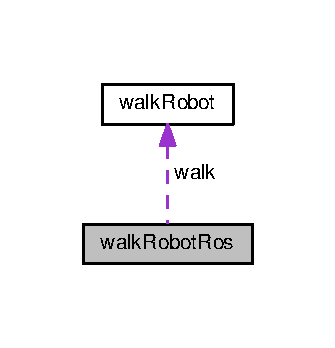
\includegraphics[width=161pt]{classwalkRobotRos__coll__graph}
\end{center}
\end{figure}
\subsection*{Public Member Functions}
\begin{DoxyCompactItemize}
\item 
\hyperlink{classwalkRobotRos_a642a5690f6c6edfcd6f0470cc59e1197}{walk\+Robot\+Ros} ()
\begin{DoxyCompactList}\small\item\em constructor of the \hyperlink{classwalkRobotRos}{walk\+Robot\+Ros} class \end{DoxyCompactList}\item 
void \hyperlink{classwalkRobotRos_ae8eb0d47c19b806f46f0bb6e50060de8}{laser\+Sensor\+Callback} (const sensor\+\_\+msgs\+::\+Laser\+Scan\+::\+Const\+Ptr \&)
\begin{DoxyCompactList}\small\item\em Sensor callback function in order to subscribe in the laser sensor topic and set the atribute obstacle in order to inform the presence or not of obstacles. \end{DoxyCompactList}\item 
void \hyperlink{classwalkRobotRos_a5fc8da4343df09e338068740bdf72b8a}{robot\+Walk\+Ros} ()
\begin{DoxyCompactList}\small\item\em Publishes msg to robot velocity. \end{DoxyCompactList}\end{DoxyCompactItemize}
\subsection*{Public Attributes}
\begin{DoxyCompactItemize}
\item 
\hyperlink{classwalkRobot}{walk\+Robot} \hyperlink{classwalkRobotRos_a52ace3b6f3d549d863de2e36faab3a46}{walk}\hypertarget{classwalkRobotRos_a52ace3b6f3d549d863de2e36faab3a46}{}\label{classwalkRobotRos_a52ace3b6f3d549d863de2e36faab3a46}

\begin{DoxyCompactList}\small\item\em Object of walk robot class. \end{DoxyCompactList}\end{DoxyCompactItemize}


\subsection{Constructor \& Destructor Documentation}
\index{walk\+Robot\+Ros@{walk\+Robot\+Ros}!walk\+Robot\+Ros@{walk\+Robot\+Ros}}
\index{walk\+Robot\+Ros@{walk\+Robot\+Ros}!walk\+Robot\+Ros@{walk\+Robot\+Ros}}
\subsubsection[{\texorpdfstring{walk\+Robot\+Ros()}{walkRobotRos()}}]{\setlength{\rightskip}{0pt plus 5cm}walk\+Robot\+Ros\+::walk\+Robot\+Ros (
\begin{DoxyParamCaption}
{}
\end{DoxyParamCaption}
)}\hypertarget{classwalkRobotRos_a642a5690f6c6edfcd6f0470cc59e1197}{}\label{classwalkRobotRos_a642a5690f6c6edfcd6f0470cc59e1197}


constructor of the \hyperlink{classwalkRobotRos}{walk\+Robot\+Ros} class 


\begin{DoxyParams}{Parameters}
{\em none} & \\
\hline
\end{DoxyParams}
\begin{DoxyReturn}{Returns}
none 
\end{DoxyReturn}
Sensor data

Advertise Velocity

seeding random number generator 

\subsection{Member Function Documentation}
\index{walk\+Robot\+Ros@{walk\+Robot\+Ros}!laser\+Sensor\+Callback@{laser\+Sensor\+Callback}}
\index{laser\+Sensor\+Callback@{laser\+Sensor\+Callback}!walk\+Robot\+Ros@{walk\+Robot\+Ros}}
\subsubsection[{\texorpdfstring{laser\+Sensor\+Callback(const sensor\+\_\+msgs\+::\+Laser\+Scan\+::\+Const\+Ptr \&)}{laserSensorCallback(const sensor_msgs::LaserScan::ConstPtr &)}}]{\setlength{\rightskip}{0pt plus 5cm}void walk\+Robot\+Ros\+::laser\+Sensor\+Callback (
\begin{DoxyParamCaption}
\item[{const sensor\+\_\+msgs\+::\+Laser\+Scan\+::\+Const\+Ptr \&}]{obs\+Msg}
\end{DoxyParamCaption}
)}\hypertarget{classwalkRobotRos_ae8eb0d47c19b806f46f0bb6e50060de8}{}\label{classwalkRobotRos_ae8eb0d47c19b806f46f0bb6e50060de8}


Sensor callback function in order to subscribe in the laser sensor topic and set the atribute obstacle in order to inform the presence or not of obstacles. 

Callback method that receives laser Scan information.


\begin{DoxyParams}{Parameters}
{\em sensor\+\_\+msgs\+::\+Laser\+Scan\+::\+Const\+Ptr} & \\
\hline
\end{DoxyParams}
\begin{DoxyReturn}{Returns}
none 
\end{DoxyReturn}
send laser scan message method of robotwalk class \index{walk\+Robot\+Ros@{walk\+Robot\+Ros}!robot\+Walk\+Ros@{robot\+Walk\+Ros}}
\index{robot\+Walk\+Ros@{robot\+Walk\+Ros}!walk\+Robot\+Ros@{walk\+Robot\+Ros}}
\subsubsection[{\texorpdfstring{robot\+Walk\+Ros()}{robotWalkRos()}}]{\setlength{\rightskip}{0pt plus 5cm}void walk\+Robot\+Ros\+::robot\+Walk\+Ros (
\begin{DoxyParamCaption}
{}
\end{DoxyParamCaption}
)}\hypertarget{classwalkRobotRos_a5fc8da4343df09e338068740bdf72b8a}{}\label{classwalkRobotRos_a5fc8da4343df09e338068740bdf72b8a}


Publishes msg to robot velocity. 

Pusblishes msg to velocity of robot.


\begin{DoxyParams}{Parameters}
{\em none} & \\
\hline
\end{DoxyParams}
\begin{DoxyReturn}{Returns}
none 
\end{DoxyReturn}


The documentation for this class was generated from the following files\+:\begin{DoxyCompactItemize}
\item 
include/\hyperlink{walkRobotRos_8hpp}{walk\+Robot\+Ros.\+hpp}\item 
src/\hyperlink{walkRobotRos_8cpp}{walk\+Robot\+Ros.\+cpp}\end{DoxyCompactItemize}

\chapter{File Documentation}
\hypertarget{collector_8hpp}{}\section{include/collector.hpp File Reference}
\label{collector_8hpp}\index{include/collector.\+hpp@{include/collector.\+hpp}}


Navigates to the marker that is to be collected.  


{\ttfamily \#include $<$ros/ros.\+h$>$}\\*
{\ttfamily \#include $<$actionlib/client/simple\+\_\+action\+\_\+client.\+h$>$}\\*
{\ttfamily \#include $<$ar\+\_\+track\+\_\+alvar\+\_\+msgs/\+Alvar\+Marker.\+h$>$}\\*
{\ttfamily \#include $<$move\+\_\+base\+\_\+msgs/\+Move\+Base\+Action.\+h$>$}\\*
{\ttfamily \#include $<$string$>$}\\*
{\ttfamily \#include $<$utility$>$}\\*
{\ttfamily \#include \char`\"{}model\+Handling.\+hpp\char`\"{}}\\*
Include dependency graph for collector.\+hpp\+:
\nopagebreak
\begin{figure}[H]
\begin{center}
\leavevmode
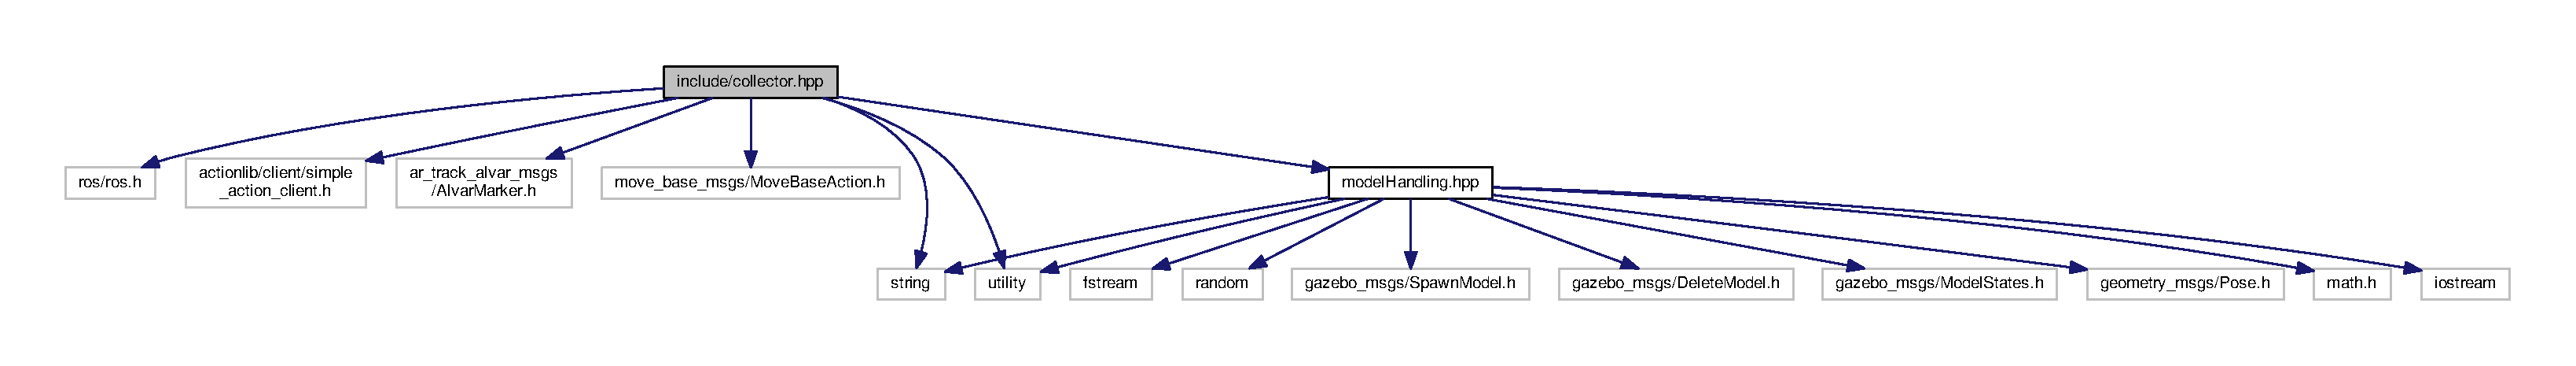
\includegraphics[width=350pt]{collector_8hpp__incl}
\end{center}
\end{figure}
This graph shows which files directly or indirectly include this file\+:
\nopagebreak
\begin{figure}[H]
\begin{center}
\leavevmode
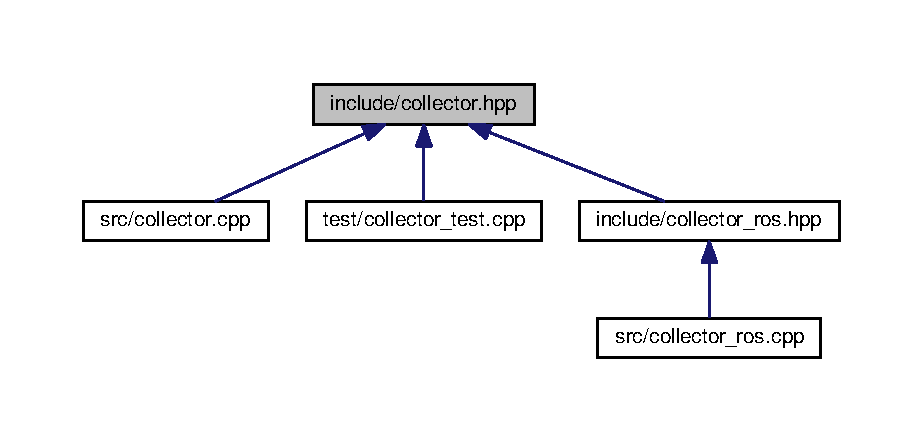
\includegraphics[width=350pt]{collector_8hpp__dep__incl}
\end{center}
\end{figure}
\subsection*{Classes}
\begin{DoxyCompactItemize}
\item 
class \hyperlink{classCollector}{Collector}
\end{DoxyCompactItemize}


\subsection{Detailed Description}
Navigates to the marker that is to be collected. 

\begin{DoxyAuthor}{Author}
Pablo Sanhueza 

Ryan Cunningham 

Andre Gomes 
\end{DoxyAuthor}
\begin{DoxyCopyright}{Copyright}
2019 Pablo Sanhueza, Andre Gomes, Ryan Cunningham 
\end{DoxyCopyright}

\hypertarget{collector__ros_8hpp}{}\section{include/collector\+\_\+ros.hpp File Reference}
\label{collector__ros_8hpp}\index{include/collector\+\_\+ros.\+hpp@{include/collector\+\_\+ros.\+hpp}}


R\+OS wrapper for the \hyperlink{classCollector}{Collector} class.  


{\ttfamily \#include $<$ros/ros.\+h$>$}\\*
{\ttfamily \#include $<$actionlib/client/simple\+\_\+action\+\_\+client.\+h$>$}\\*
{\ttfamily \#include $<$ar\+\_\+track\+\_\+alvar\+\_\+msgs/\+Alvar\+Marker.\+h$>$}\\*
{\ttfamily \#include $<$move\+\_\+base\+\_\+msgs/\+Move\+Base\+Action.\+h$>$}\\*
{\ttfamily \#include $<$string$>$}\\*
{\ttfamily \#include \char`\"{}model\+Handling.\+hpp\char`\"{}}\\*
{\ttfamily \#include \char`\"{}collector.\+hpp\char`\"{}}\\*
Include dependency graph for collector\+\_\+ros.\+hpp\+:
\nopagebreak
\begin{figure}[H]
\begin{center}
\leavevmode
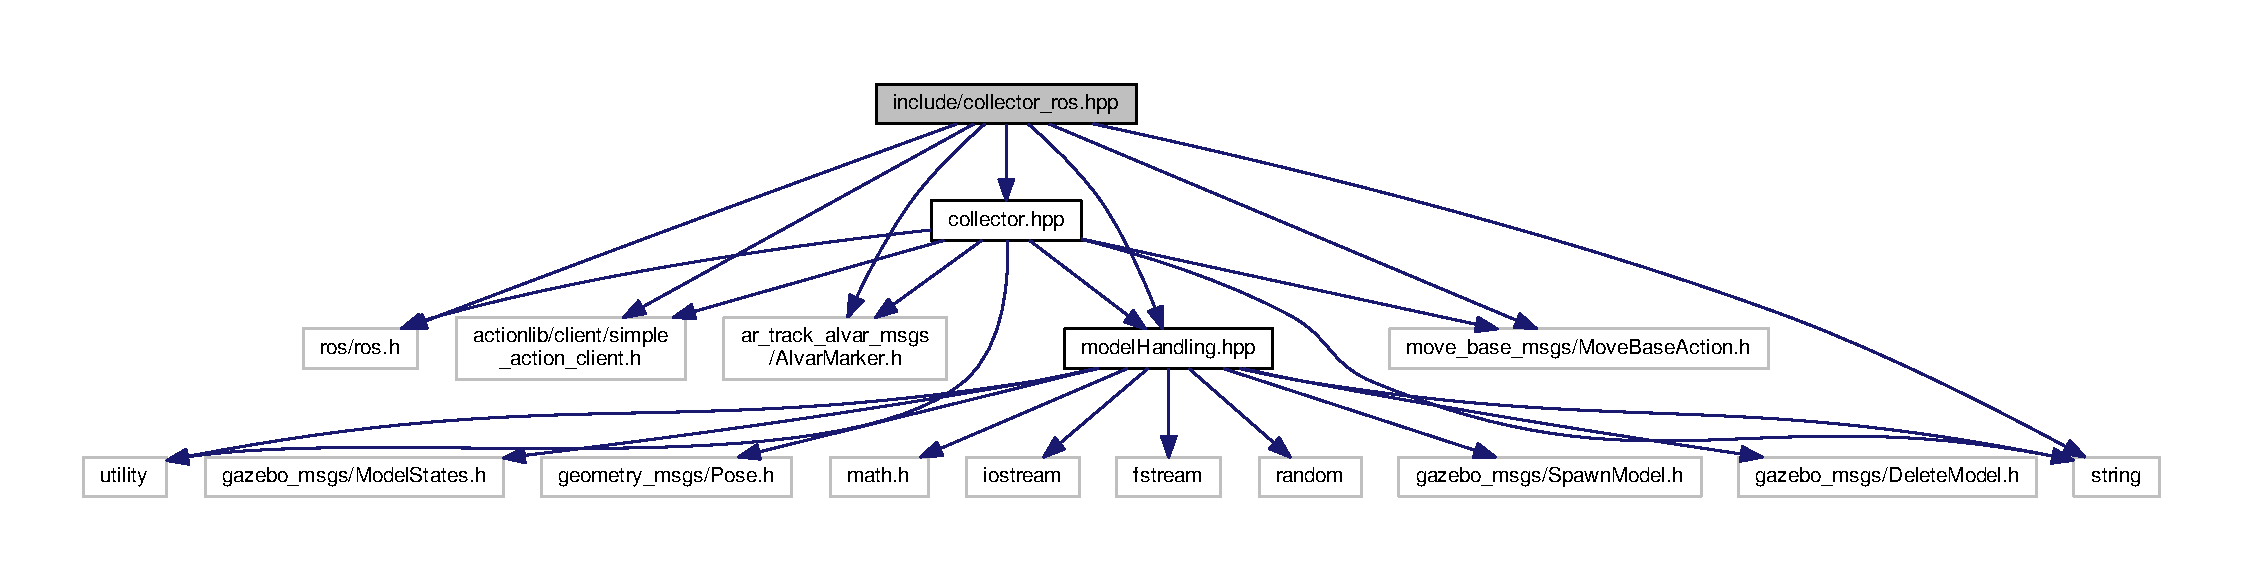
\includegraphics[width=350pt]{collector__ros_8hpp__incl}
\end{center}
\end{figure}
This graph shows which files directly or indirectly include this file\+:
\nopagebreak
\begin{figure}[H]
\begin{center}
\leavevmode
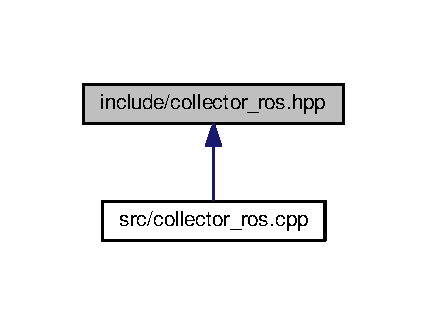
\includegraphics[width=205pt]{collector__ros_8hpp__dep__incl}
\end{center}
\end{figure}
\subsection*{Classes}
\begin{DoxyCompactItemize}
\item 
class \hyperlink{classCollectorRos}{Collector\+Ros}
\end{DoxyCompactItemize}


\subsection{Detailed Description}
R\+OS wrapper for the \hyperlink{classCollector}{Collector} class. 

\begin{DoxyAuthor}{Author}
Pablo Sanhueza 

Ryan Cunningham 

Andre Gomes 
\end{DoxyAuthor}
\begin{DoxyCopyright}{Copyright}
2019 Pablo Sanhueza, Andre Gomes, Ryan Cunningham 
\end{DoxyCopyright}

\hypertarget{detector_8hpp}{}\section{include/detector.hpp File Reference}
\label{detector_8hpp}\index{include/detector.\+hpp@{include/detector.\+hpp}}


Detects the closest AR tag.  


{\ttfamily \#include $<$ros/ros.\+h$>$}\\*
{\ttfamily \#include $<$ar\+\_\+track\+\_\+alvar\+\_\+msgs/\+Alvar\+Markers.\+h$>$}\\*
{\ttfamily \#include $<$ar\+\_\+track\+\_\+alvar\+\_\+msgs/\+Alvar\+Marker.\+h$>$}\\*
{\ttfamily \#include $<$string$>$}\\*
{\ttfamily \#include $<$vector$>$}\\*
Include dependency graph for detector.\+hpp\+:
\nopagebreak
\begin{figure}[H]
\begin{center}
\leavevmode
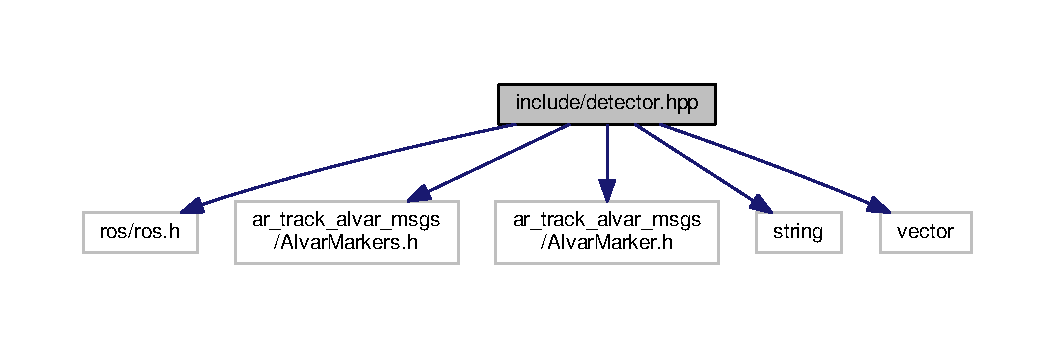
\includegraphics[width=350pt]{detector_8hpp__incl}
\end{center}
\end{figure}
This graph shows which files directly or indirectly include this file\+:
\nopagebreak
\begin{figure}[H]
\begin{center}
\leavevmode
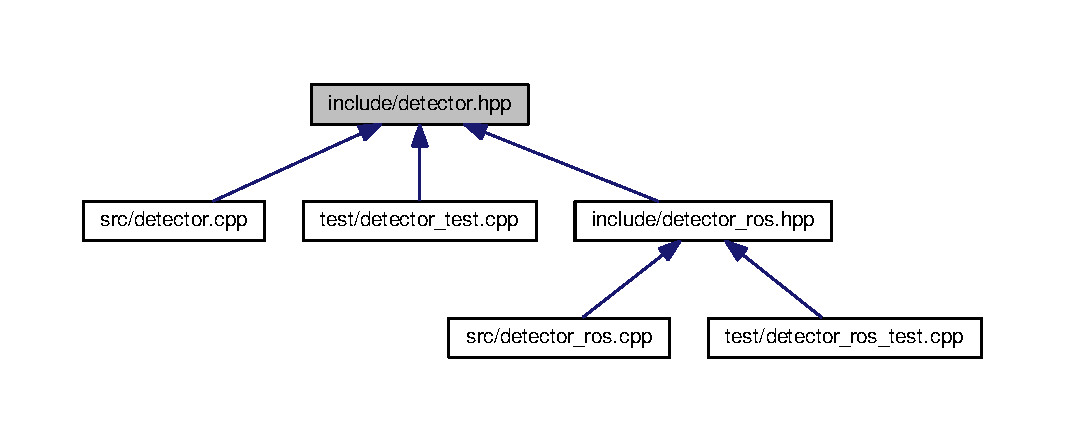
\includegraphics[width=350pt]{detector_8hpp__dep__incl}
\end{center}
\end{figure}
\subsection*{Classes}
\begin{DoxyCompactItemize}
\item 
class \hyperlink{classDetector}{Detector}
\begin{DoxyCompactList}\small\item\em Detects AR tags. \end{DoxyCompactList}\end{DoxyCompactItemize}


\subsection{Detailed Description}
Detects the closest AR tag. 

\begin{DoxyAuthor}{Author}
Pablo Sanhueza 

Ryan Cunningham 

Andre Gomes 
\end{DoxyAuthor}
\begin{DoxyCopyright}{Copyright}
2019 Pablo Sanhueza, Andre Gomes, Ryan Cunningham 
\end{DoxyCopyright}

\hypertarget{detector__ros_8hpp}{}\section{include/detector\+\_\+ros.hpp File Reference}
\label{detector__ros_8hpp}\index{include/detector\+\_\+ros.\+hpp@{include/detector\+\_\+ros.\+hpp}}


R\+OS wrapper for he \hyperlink{classDetectorRos}{Detector\+Ros} class.  


{\ttfamily \#include $<$ros/ros.\+h$>$}\\*
{\ttfamily \#include $<$ar\+\_\+track\+\_\+alvar\+\_\+msgs/\+Alvar\+Markers.\+h$>$}\\*
{\ttfamily \#include $<$ar\+\_\+track\+\_\+alvar\+\_\+msgs/\+Alvar\+Marker.\+h$>$}\\*
{\ttfamily \#include $<$string$>$}\\*
{\ttfamily \#include $<$vector$>$}\\*
{\ttfamily \#include \char`\"{}detector.\+hpp\char`\"{}}\\*
Include dependency graph for detector\+\_\+ros.\+hpp\+:
\nopagebreak
\begin{figure}[H]
\begin{center}
\leavevmode
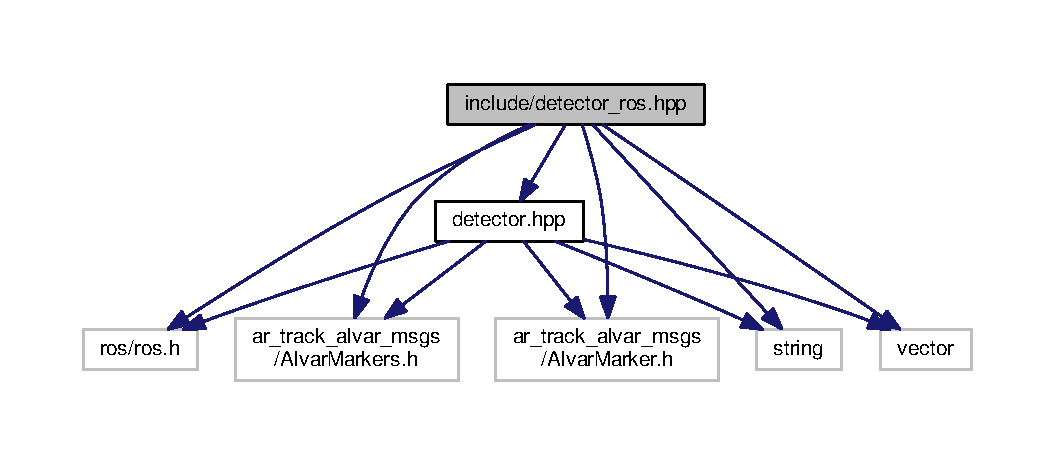
\includegraphics[width=350pt]{detector__ros_8hpp__incl}
\end{center}
\end{figure}
This graph shows which files directly or indirectly include this file\+:
\nopagebreak
\begin{figure}[H]
\begin{center}
\leavevmode
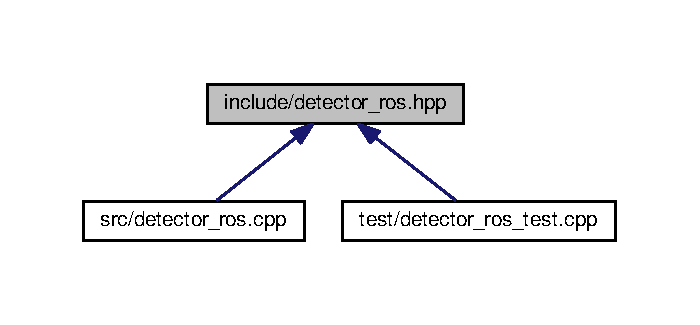
\includegraphics[width=336pt]{detector__ros_8hpp__dep__incl}
\end{center}
\end{figure}
\subsection*{Classes}
\begin{DoxyCompactItemize}
\item 
class \hyperlink{classDetectorRos}{Detector\+Ros}
\begin{DoxyCompactList}\small\item\em Detects AR tags. \end{DoxyCompactList}\end{DoxyCompactItemize}


\subsection{Detailed Description}
R\+OS wrapper for he \hyperlink{classDetectorRos}{Detector\+Ros} class. 

\begin{DoxyAuthor}{Author}
Pablo Sanhueza 

Ryan Cunningham 

Andre Gomes 
\end{DoxyAuthor}
\begin{DoxyCopyright}{Copyright}
2019 Pablo Sanhueza, Andre Gomes, Ryan Cunningham 
\end{DoxyCopyright}

\hypertarget{walkRobot_8hpp}{}\section{include/walk\+Robot.hpp File Reference}
\label{walkRobot_8hpp}\index{include/walk\+Robot.\+hpp@{include/walk\+Robot.\+hpp}}


Declaring class \hyperlink{classwalkRobot}{walk\+Robot}.  


{\ttfamily \#include $<$ros/ros.\+h$>$}\\*
{\ttfamily \#include $<$sensor\+\_\+msgs/\+Laser\+Scan.\+h$>$}\\*
{\ttfamily \#include \char`\"{}geometry\+\_\+msgs/\+Twist.\+h\char`\"{}}\\*
Include dependency graph for walk\+Robot.\+hpp\+:
\nopagebreak
\begin{figure}[H]
\begin{center}
\leavevmode
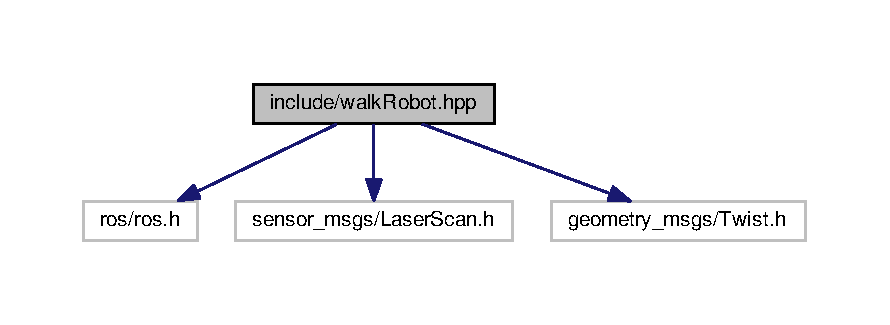
\includegraphics[width=350pt]{walkRobot_8hpp__incl}
\end{center}
\end{figure}
This graph shows which files directly or indirectly include this file\+:
\nopagebreak
\begin{figure}[H]
\begin{center}
\leavevmode
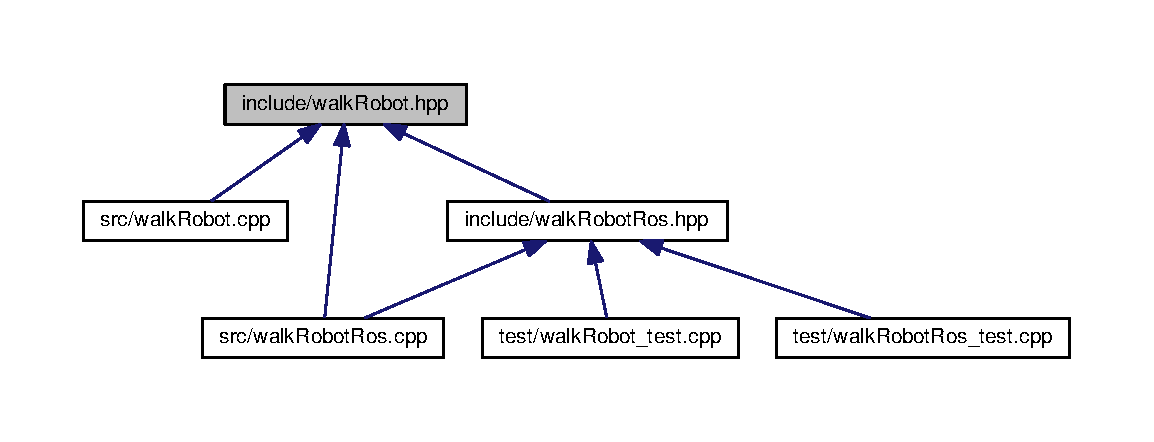
\includegraphics[width=350pt]{walkRobot_8hpp__dep__incl}
\end{center}
\end{figure}
\subsection*{Classes}
\begin{DoxyCompactItemize}
\item 
class \hyperlink{classwalkRobot}{walk\+Robot}
\end{DoxyCompactItemize}


\subsection{Detailed Description}
Declaring class \hyperlink{classwalkRobot}{walk\+Robot}. 

/$\ast$ This Source Code Form is subject to the terms of the Mozilla Public License, v. 2.\+0. If a copy of the M\+PL was not distributed with this file, You can obtain one at \href{https://mozilla.org/MPL/2.0/}{\tt https\+://mozilla.\+org/\+M\+P\+L/2.\+0/}.

\begin{DoxyAuthor}{Author}
Pablo Sanhueza, Ryan Cunningham, Andre Gomes 
\end{DoxyAuthor}
\begin{DoxyCopyright}{Copyright}
2019 Pablo Sanhueza, Ryan Cunningham, Andre Gomes 
\end{DoxyCopyright}

\hypertarget{walkRobotRos_8hpp}{}\section{include/walk\+Robot\+Ros.hpp File Reference}
\label{walkRobotRos_8hpp}\index{include/walk\+Robot\+Ros.\+hpp@{include/walk\+Robot\+Ros.\+hpp}}


Declaring class \hyperlink{classwalkRobotRos}{walk\+Robot\+Ros}.  


{\ttfamily \#include $<$ros/ros.\+h$>$}\\*
{\ttfamily \#include $<$sensor\+\_\+msgs/\+Laser\+Scan.\+h$>$}\\*
{\ttfamily \#include \char`\"{}geometry\+\_\+msgs/\+Twist.\+h\char`\"{}}\\*
{\ttfamily \#include \char`\"{}walk\+Robot.\+hpp\char`\"{}}\\*
Include dependency graph for walk\+Robot\+Ros.\+hpp\+:
\nopagebreak
\begin{figure}[H]
\begin{center}
\leavevmode
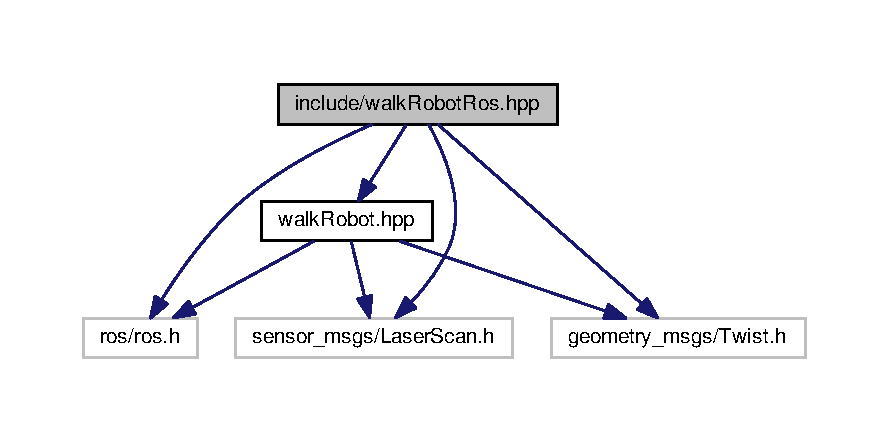
\includegraphics[width=350pt]{walkRobotRos_8hpp__incl}
\end{center}
\end{figure}
This graph shows which files directly or indirectly include this file\+:
\nopagebreak
\begin{figure}[H]
\begin{center}
\leavevmode
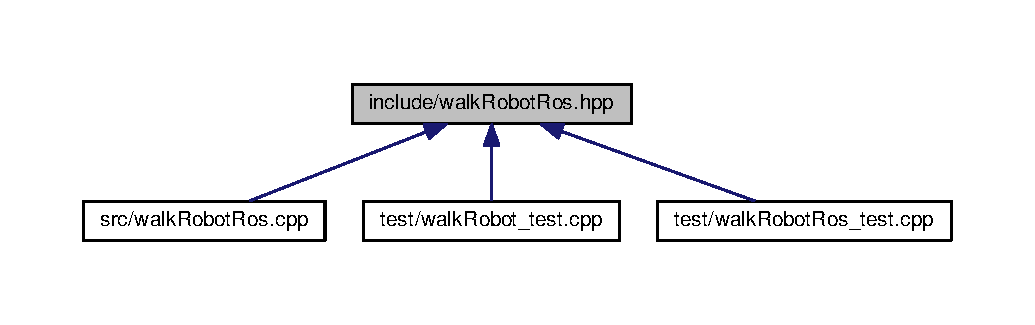
\includegraphics[width=350pt]{walkRobotRos_8hpp__dep__incl}
\end{center}
\end{figure}
\subsection*{Classes}
\begin{DoxyCompactItemize}
\item 
class \hyperlink{classwalkRobotRos}{walk\+Robot\+Ros}
\end{DoxyCompactItemize}


\subsection{Detailed Description}
Declaring class \hyperlink{classwalkRobotRos}{walk\+Robot\+Ros}. 

/$\ast$ This Source Code Form is subject to the terms of the Mozilla Public License, v. 2.\+0. If a copy of the M\+PL was not distributed with this file, You can obtain one at \href{https://mozilla.org/MPL/2.0/}{\tt https\+://mozilla.\+org/\+M\+P\+L/2.\+0/}.

\begin{DoxyAuthor}{Author}
Pablo Sanhueza, Ryan Cunningham, Andre Gomes 
\end{DoxyAuthor}
\begin{DoxyCopyright}{Copyright}
2019 Pablo Sanhueza, Ryan Cunningham, Andre Gomes 
\end{DoxyCopyright}

\hypertarget{collector_8cpp}{}\section{src/collector.cpp File Reference}
\label{collector_8cpp}\index{src/collector.\+cpp@{src/collector.\+cpp}}


Navigates to the marker that is to be collected.  


{\ttfamily \#include \char`\"{}collector.\+hpp\char`\"{}}\\*
{\ttfamily \#include $<$actionlib/client/simple\+\_\+action\+\_\+client.\+h$>$}\\*
{\ttfamily \#include $<$ar\+\_\+track\+\_\+alvar\+\_\+msgs/\+Alvar\+Marker.\+h$>$}\\*
{\ttfamily \#include $<$move\+\_\+base\+\_\+msgs/\+Move\+Base\+Action.\+h$>$}\\*
{\ttfamily \#include $<$tf/tf.\+h$>$}\\*
{\ttfamily \#include $<$string$>$}\\*
{\ttfamily \#include \char`\"{}model\+Handling.\+hpp\char`\"{}}\\*
Include dependency graph for collector.\+cpp\+:
\nopagebreak
\begin{figure}[H]
\begin{center}
\leavevmode
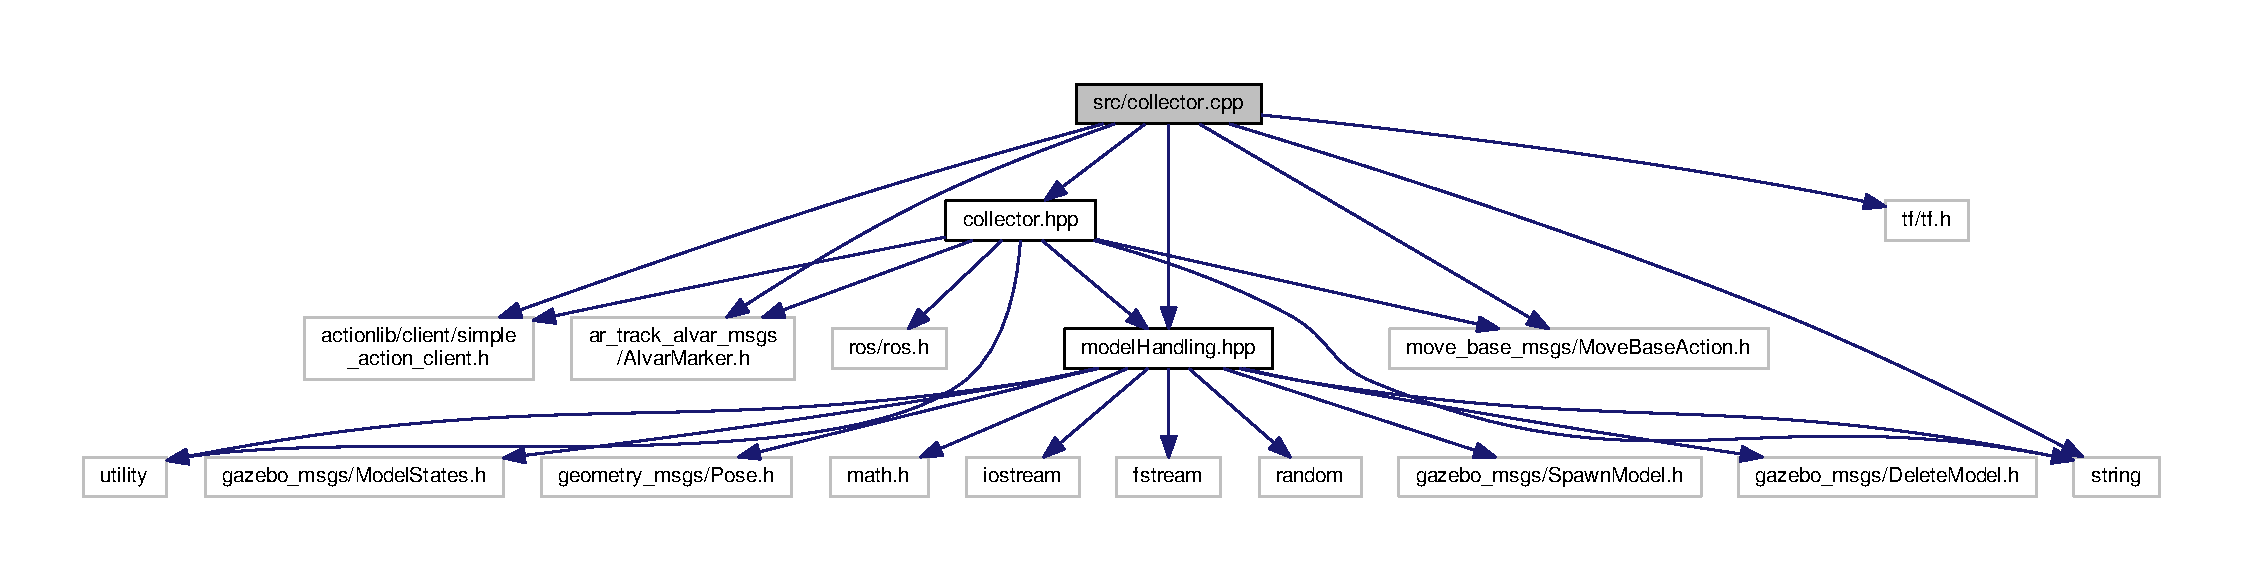
\includegraphics[width=350pt]{collector_8cpp__incl}
\end{center}
\end{figure}


\subsection{Detailed Description}
Navigates to the marker that is to be collected. 

This Source Code Form is subject to the terms of the Mozilla Public License, v. 2.\+0. If a copy of the M\+PL was not distributed with this file, You can obtain one at \href{https://mozilla.org/MPL/2.0/}{\tt https\+://mozilla.\+org/\+M\+P\+L/2.\+0/}.

\begin{DoxyAuthor}{Author}
Pablo Sanhueza, Ryan Cunningham, Andre Gomes 
\end{DoxyAuthor}
\begin{DoxyCopyright}{Copyright}
2019 Pablo Sanhueza, Andre Gomes, Ryan Cunningham 
\end{DoxyCopyright}

\hypertarget{collector__ros_8cpp}{}\section{src/collector\+\_\+ros.cpp File Reference}
\label{collector__ros_8cpp}\index{src/collector\+\_\+ros.\+cpp@{src/collector\+\_\+ros.\+cpp}}


R\+OS wrapper for the \hyperlink{classCollector}{Collector} class.  


{\ttfamily \#include \char`\"{}collector\+\_\+ros.\+hpp\char`\"{}}\\*
{\ttfamily \#include $<$actionlib/client/simple\+\_\+action\+\_\+client.\+h$>$}\\*
{\ttfamily \#include $<$ar\+\_\+track\+\_\+alvar\+\_\+msgs/\+Alvar\+Marker.\+h$>$}\\*
{\ttfamily \#include $<$move\+\_\+base\+\_\+msgs/\+Move\+Base\+Action.\+h$>$}\\*
{\ttfamily \#include $<$tf/tf.\+h$>$}\\*
{\ttfamily \#include $<$string$>$}\\*
{\ttfamily \#include \char`\"{}model\+Handling.\+hpp\char`\"{}}\\*
Include dependency graph for collector\+\_\+ros.\+cpp\+:
\nopagebreak
\begin{figure}[H]
\begin{center}
\leavevmode
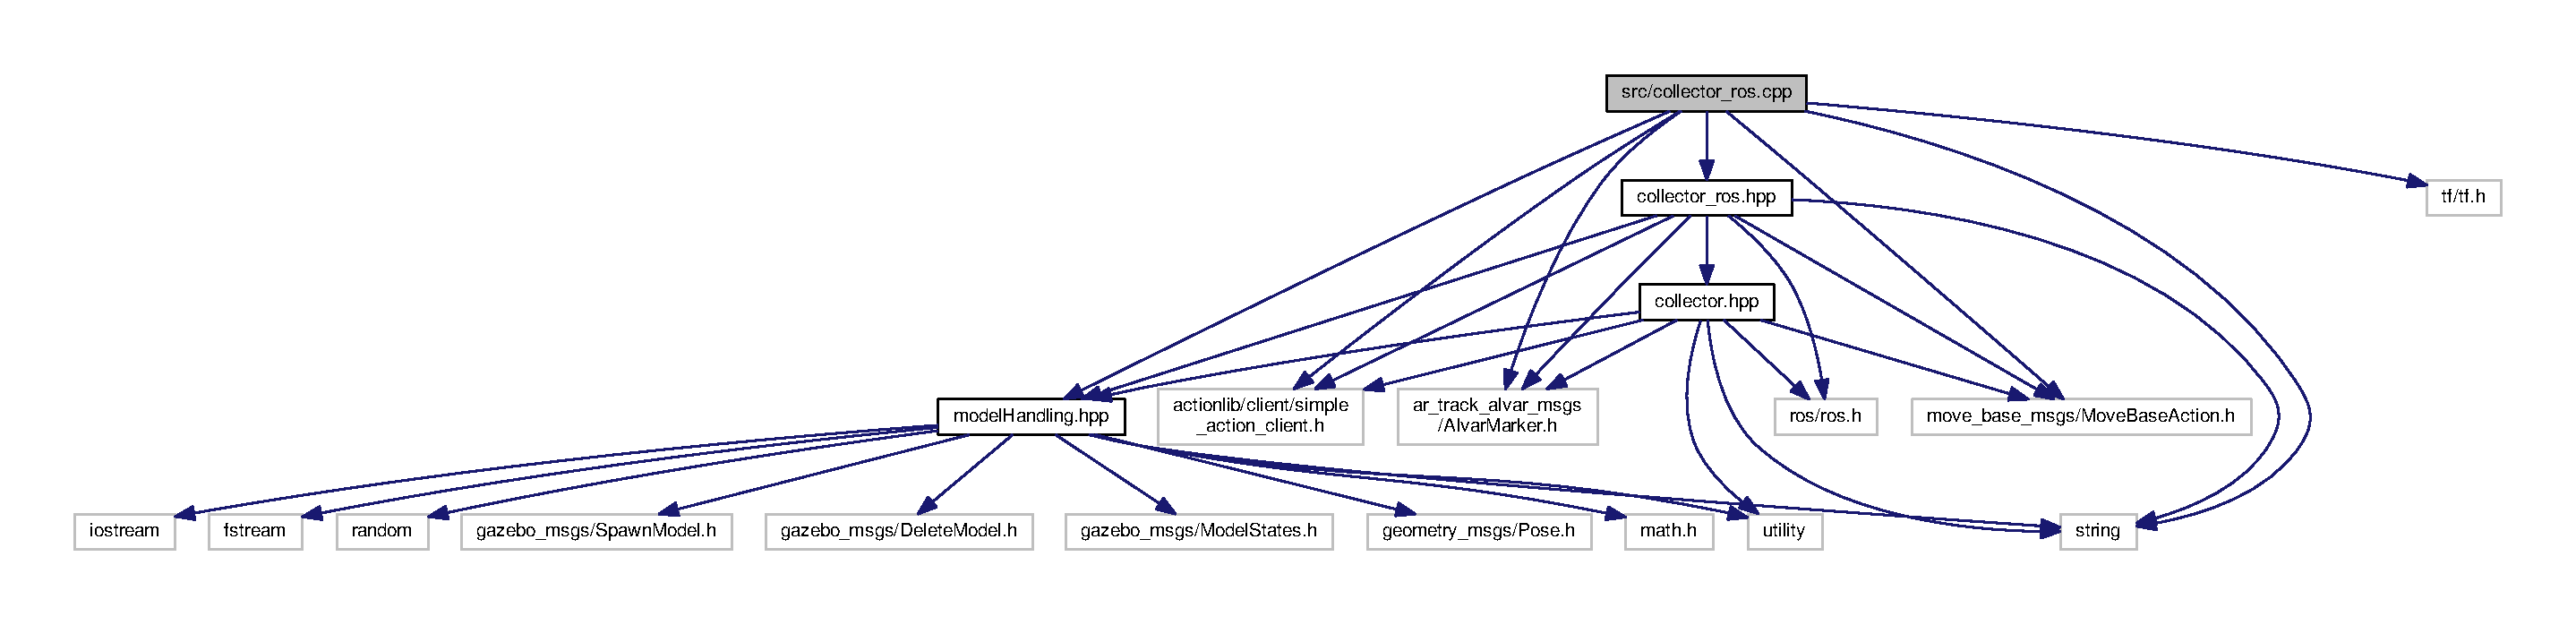
\includegraphics[width=350pt]{collector__ros_8cpp__incl}
\end{center}
\end{figure}


\subsection{Detailed Description}
R\+OS wrapper for the \hyperlink{classCollector}{Collector} class. 

This Source Code Form is subject to the terms of the Mozilla Public License, v. 2.\+0. If a copy of the M\+PL was not distributed with this file, You can obtain one at \href{https://mozilla.org/MPL/2.0/}{\tt https\+://mozilla.\+org/\+M\+P\+L/2.\+0/}.

\begin{DoxyAuthor}{Author}
Pablo Sanhueza, Ryan Cunningham, Andre Gomes 
\end{DoxyAuthor}
\begin{DoxyCopyright}{Copyright}
2019 Pablo Sanhueza, Andre Gomes, Ryan Cunningham 
\end{DoxyCopyright}

\hypertarget{detector_8cpp}{}\section{src/detector.cpp File Reference}
\label{detector_8cpp}\index{src/detector.\+cpp@{src/detector.\+cpp}}


Detects the closest AR tag.  


{\ttfamily \#include \char`\"{}detector.\+hpp\char`\"{}}\\*
{\ttfamily \#include $<$ar\+\_\+track\+\_\+alvar\+\_\+msgs/\+Alvar\+Markers.\+h$>$}\\*
{\ttfamily \#include $<$ar\+\_\+track\+\_\+alvar\+\_\+msgs/\+Alvar\+Marker.\+h$>$}\\*
{\ttfamily \#include $<$math.\+h$>$}\\*
Include dependency graph for detector.\+cpp\+:
\nopagebreak
\begin{figure}[H]
\begin{center}
\leavevmode
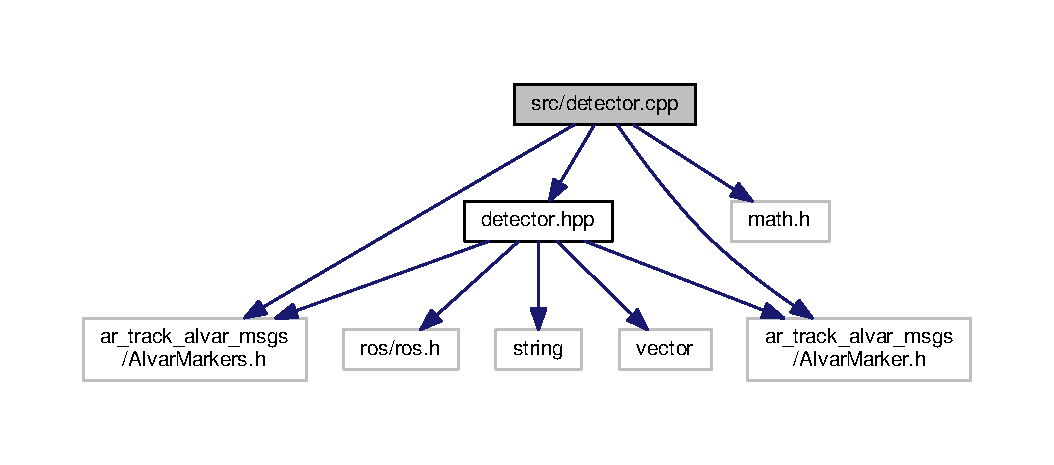
\includegraphics[width=350pt]{detector_8cpp__incl}
\end{center}
\end{figure}


\subsection{Detailed Description}
Detects the closest AR tag. 

This Source Code Form is subject to the terms of the Mozilla Public License, v. 2.\+0. If a copy of the M\+PL was not distributed with this file, You can obtain one at \href{https://mozilla.org/MPL/2.0/}{\tt https\+://mozilla.\+org/\+M\+P\+L/2.\+0/}.

\begin{DoxyAuthor}{Author}
Pablo Sanhueza, Ryan Cunningham, Andre Gomes 
\end{DoxyAuthor}
\begin{DoxyCopyright}{Copyright}
2019 Pablo Sanhueza, Andre Gomes, Ryan Cunningham 
\end{DoxyCopyright}

\hypertarget{detector__ros_8cpp}{}\section{src/detector\+\_\+ros.cpp File Reference}
\label{detector__ros_8cpp}\index{src/detector\+\_\+ros.\+cpp@{src/detector\+\_\+ros.\+cpp}}


R\+OS wrapper for the \hyperlink{classDetectorRos}{Detector\+Ros} class.  


{\ttfamily \#include \char`\"{}detector\+\_\+ros.\+hpp\char`\"{}}\\*
{\ttfamily \#include $<$ar\+\_\+track\+\_\+alvar\+\_\+msgs/\+Alvar\+Markers.\+h$>$}\\*
{\ttfamily \#include $<$ar\+\_\+track\+\_\+alvar\+\_\+msgs/\+Alvar\+Marker.\+h$>$}\\*
{\ttfamily \#include $<$math.\+h$>$}\\*
Include dependency graph for detector\+\_\+ros.\+cpp\+:
\nopagebreak
\begin{figure}[H]
\begin{center}
\leavevmode
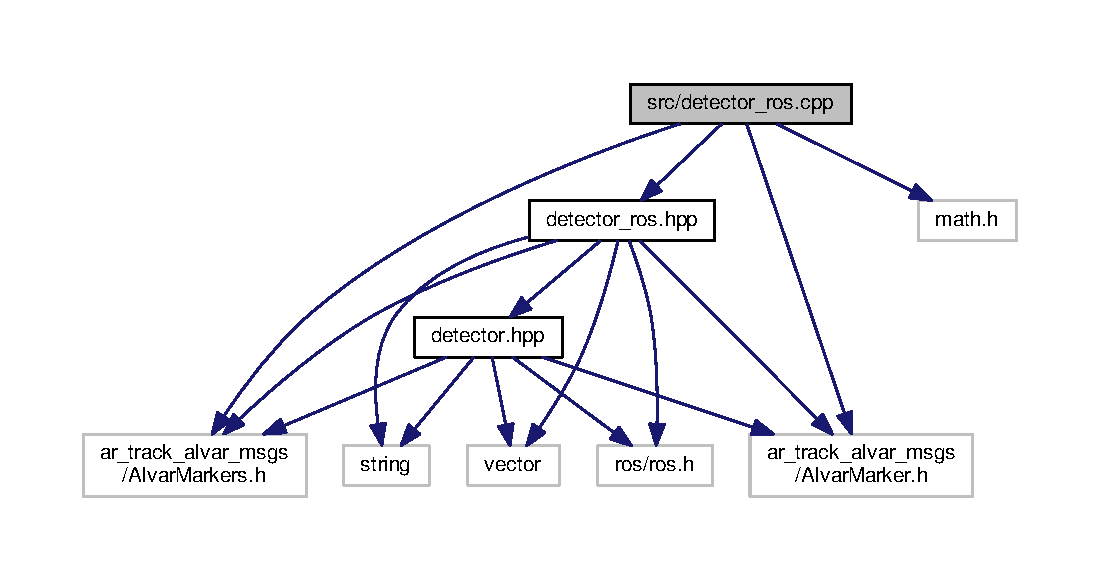
\includegraphics[width=350pt]{detector__ros_8cpp__incl}
\end{center}
\end{figure}


\subsection{Detailed Description}
R\+OS wrapper for the \hyperlink{classDetectorRos}{Detector\+Ros} class. 

This Source Code Form is subject to the terms of the Mozilla Public License, v. 2.\+0. If a copy of the M\+PL was not distributed with this file, You can obtain one at \href{https://mozilla.org/MPL/2.0/}{\tt https\+://mozilla.\+org/\+M\+P\+L/2.\+0/}.

\begin{DoxyAuthor}{Author}
Pablo Sanhueza, Ryan Cunningham, Andre Gomes 
\end{DoxyAuthor}
\begin{DoxyCopyright}{Copyright}
2019 Pablo Sanhueza, Andre Gomes, Ryan Cunningham 
\end{DoxyCopyright}

\hypertarget{walkRobot_8cpp}{}\section{src/walk\+Robot.cpp File Reference}
\label{walkRobot_8cpp}\index{src/walk\+Robot.\+cpp@{src/walk\+Robot.\+cpp}}


Source code for the implementation of \hyperlink{classwalkRobot}{walk\+Robot} class.  


{\ttfamily \#include \char`\"{}walk\+Robot.\+hpp\char`\"{}}\\*
{\ttfamily \#include $<$stdlib.\+h$>$}\\*
{\ttfamily \#include $<$ros/ros.\+h$>$}\\*
{\ttfamily \#include $<$time.\+h$>$}\\*
{\ttfamily \#include $<$sensor\+\_\+msgs/\+Laser\+Scan.\+h$>$}\\*
{\ttfamily \#include \char`\"{}geometry\+\_\+msgs/\+Twist.\+h\char`\"{}}\\*
Include dependency graph for walk\+Robot.\+cpp\+:
\nopagebreak
\begin{figure}[H]
\begin{center}
\leavevmode
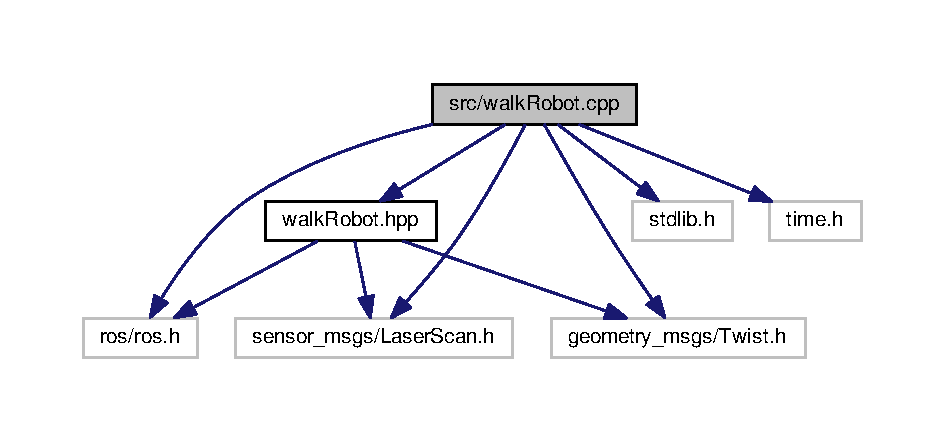
\includegraphics[width=350pt]{walkRobot_8cpp__incl}
\end{center}
\end{figure}


\subsection{Detailed Description}
Source code for the implementation of \hyperlink{classwalkRobot}{walk\+Robot} class. 

/$\ast$ This Source Code Form is subject to the terms of the Mozilla Public License, v. 2.\+0. If a copy of the M\+PL was not distributed with this file, You can obtain one at \href{https://mozilla.org/MPL/2.0/}{\tt https\+://mozilla.\+org/\+M\+P\+L/2.\+0/}.

\begin{DoxyAuthor}{Author}
Pablo Sanhueza, Ryan Cunningham, Andre Gomes 
\end{DoxyAuthor}
\begin{DoxyCopyright}{Copyright}
2019 Pablo Sanhueza, Ryan Cunningham, Andre Gomes 
\end{DoxyCopyright}

\hypertarget{walkRobotRos_8cpp}{}\section{src/walk\+Robot\+Ros.cpp File Reference}
\label{walkRobotRos_8cpp}\index{src/walk\+Robot\+Ros.\+cpp@{src/walk\+Robot\+Ros.\+cpp}}


Source code for the implementation of \hyperlink{classwalkRobotRos}{walk\+Robot\+Ros} class.  


{\ttfamily \#include \char`\"{}walk\+Robot\+Ros.\+hpp\char`\"{}}\\*
{\ttfamily \#include $<$stdlib.\+h$>$}\\*
{\ttfamily \#include $<$ros/ros.\+h$>$}\\*
{\ttfamily \#include $<$time.\+h$>$}\\*
{\ttfamily \#include $<$sensor\+\_\+msgs/\+Laser\+Scan.\+h$>$}\\*
{\ttfamily \#include \char`\"{}geometry\+\_\+msgs/\+Twist.\+h\char`\"{}}\\*
{\ttfamily \#include \char`\"{}walk\+Robot.\+hpp\char`\"{}}\\*
Include dependency graph for walk\+Robot\+Ros.\+cpp\+:
\nopagebreak
\begin{figure}[H]
\begin{center}
\leavevmode
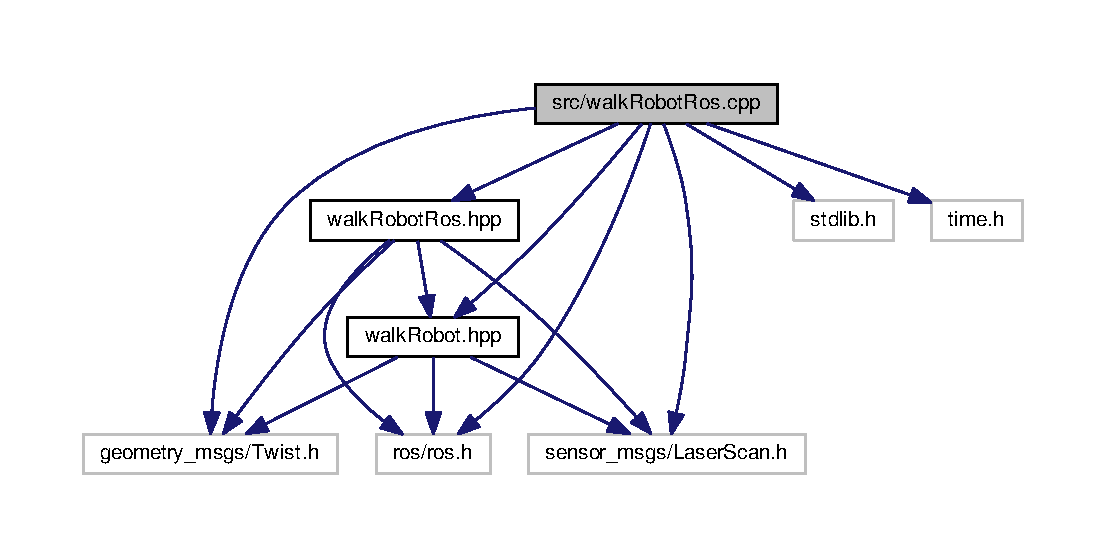
\includegraphics[width=350pt]{walkRobotRos_8cpp__incl}
\end{center}
\end{figure}


\subsection{Detailed Description}
Source code for the implementation of \hyperlink{classwalkRobotRos}{walk\+Robot\+Ros} class. 

/$\ast$ This Source Code Form is subject to the terms of the Mozilla Public License, v. 2.\+0. If a copy of the M\+PL was not distributed with this file, You can obtain one at \href{https://mozilla.org/MPL/2.0/}{\tt https\+://mozilla.\+org/\+M\+P\+L/2.\+0/}.

\begin{DoxyAuthor}{Author}
Pablo Sanhueza, Ryan Cunningham, Andre Gomes 
\end{DoxyAuthor}
\begin{DoxyCopyright}{Copyright}
2019 Pablo Sanhueza, Ryan Cunningham, Andre Gomes 
\end{DoxyCopyright}

\hypertarget{collector__test_8cpp}{}\section{test/collector\+\_\+test.cpp File Reference}
\label{collector__test_8cpp}\index{test/collector\+\_\+test.\+cpp@{test/collector\+\_\+test.\+cpp}}
{\ttfamily \#include \char`\"{}collector.\+hpp\char`\"{}}\\*
{\ttfamily \#include $<$gtest/gtest.\+h$>$}\\*
Include dependency graph for collector\+\_\+test.\+cpp\+:
\nopagebreak
\begin{figure}[H]
\begin{center}
\leavevmode
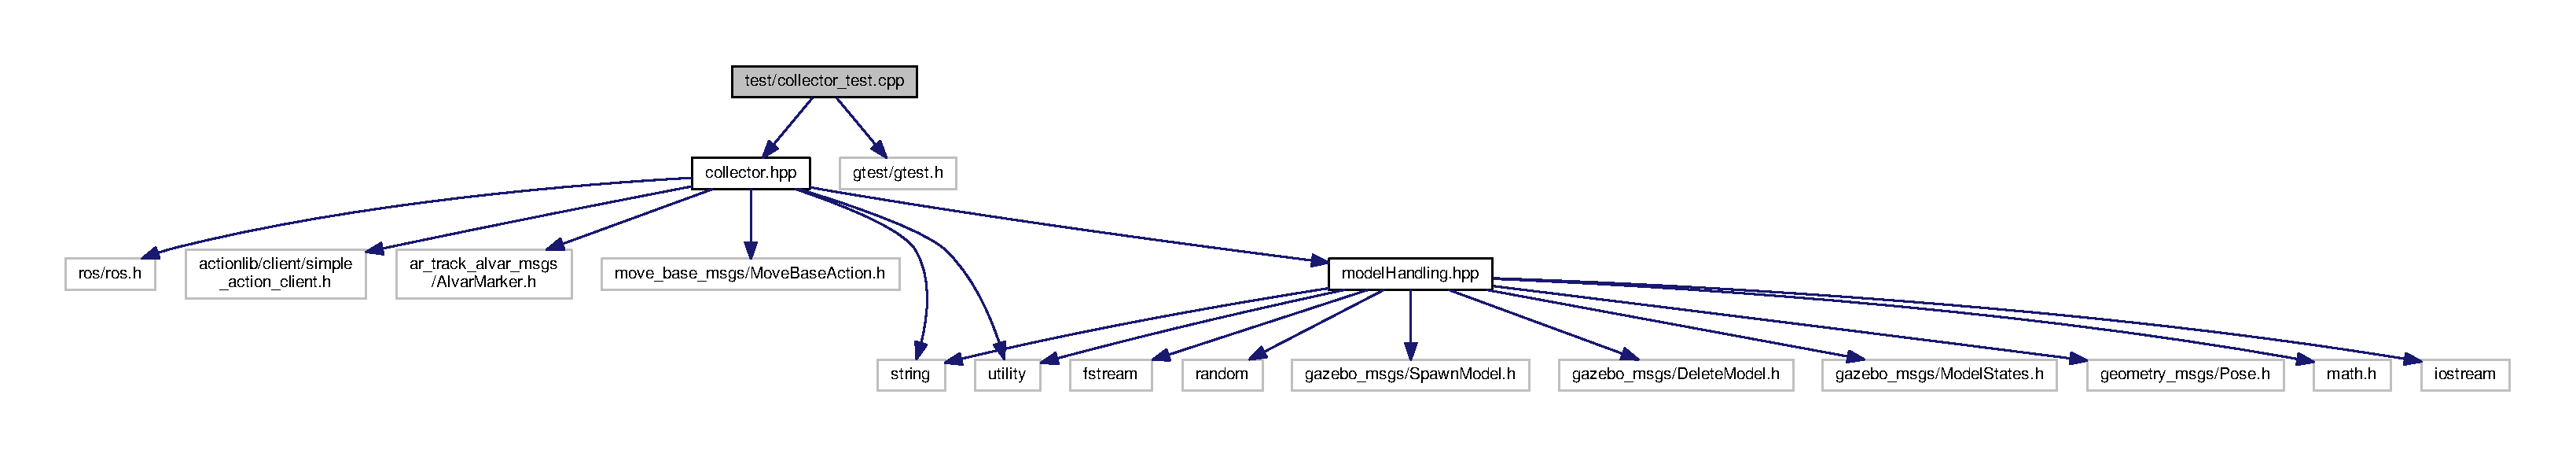
\includegraphics[width=350pt]{collector__test_8cpp__incl}
\end{center}
\end{figure}
\subsection*{Functions}
\begin{DoxyCompactItemize}
\item 
{\bfseries T\+E\+ST} (Collector\+Test, test\+Create\+Move\+Base\+Goal)\hypertarget{collector__test_8cpp_a3fba7bcf14b6dcacb9dda85c8e539335}{}\label{collector__test_8cpp_a3fba7bcf14b6dcacb9dda85c8e539335}

\item 
{\bfseries T\+E\+ST} (Collector\+Test, test\+Translate\+Point\+To\+Origin)\hypertarget{collector__test_8cpp_a3c104aa14ac9e9f2d6dcd8a50c12c423}{}\label{collector__test_8cpp_a3c104aa14ac9e9f2d6dcd8a50c12c423}

\end{DoxyCompactItemize}


\subsection{Detailed Description}
\begin{DoxyCopyright}{Copyright}
2019 
\end{DoxyCopyright}

\hypertarget{detector__ros__test_8cpp}{}\section{test/detector\+\_\+ros\+\_\+test.cpp File Reference}
\label{detector__ros__test_8cpp}\index{test/detector\+\_\+ros\+\_\+test.\+cpp@{test/detector\+\_\+ros\+\_\+test.\+cpp}}


Unit Test for \hyperlink{classDetectorRos}{Detector\+Ros} class.  


{\ttfamily \#include \char`\"{}detector\+\_\+ros.\+hpp\char`\"{}}\\*
{\ttfamily \#include $<$ar\+\_\+track\+\_\+alvar\+\_\+msgs/\+Alvar\+Markers.\+h$>$}\\*
{\ttfamily \#include $<$ar\+\_\+track\+\_\+alvar\+\_\+msgs/\+Alvar\+Marker.\+h$>$}\\*
{\ttfamily \#include $<$gtest/gtest.\+h$>$}\\*
{\ttfamily \#include $<$ros/ros.\+h$>$}\\*
Include dependency graph for detector\+\_\+ros\+\_\+test.\+cpp\+:
\nopagebreak
\begin{figure}[H]
\begin{center}
\leavevmode
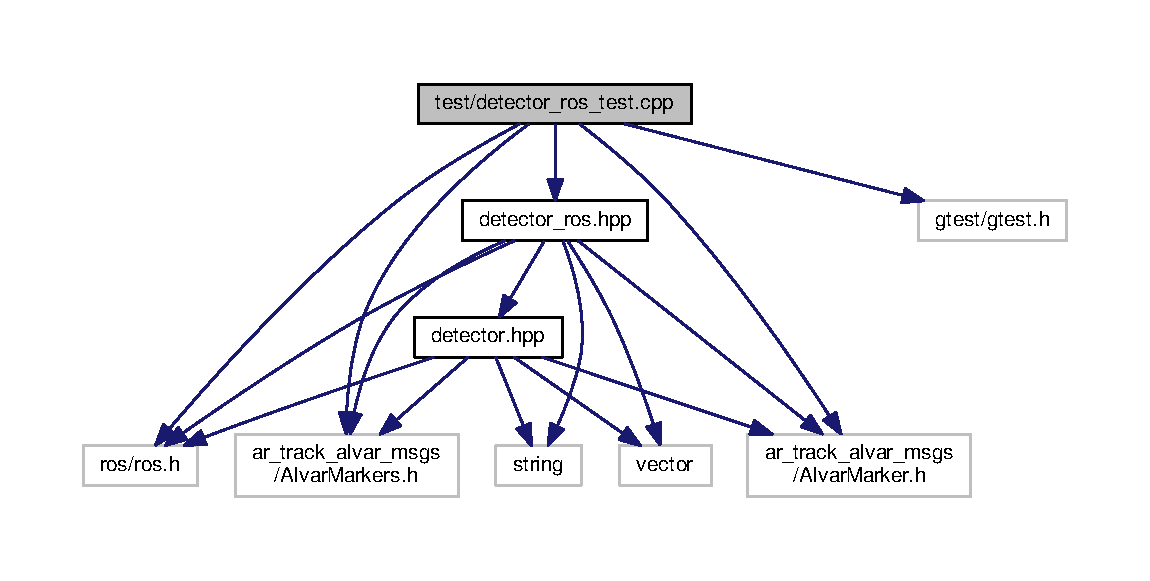
\includegraphics[width=350pt]{detector__ros__test_8cpp__incl}
\end{center}
\end{figure}
\subsection*{Functions}
\begin{DoxyCompactItemize}
\item 
\hyperlink{detector__ros__test_8cpp_aad4b6204a848a52b8161439ce5b73769}{T\+E\+ST} (Detector\+Ros\+Test, test\+No\+Detected\+Markers)
\begin{DoxyCompactList}\small\item\em Test that no markers are detected when a message is published that has no markers. \end{DoxyCompactList}\item 
\hyperlink{detector__ros__test_8cpp_a780d4683628736d76be512db6ff54e73}{T\+E\+ST} (Detector\+Ros\+Test, test\+Detected\+Markers)
\begin{DoxyCompactList}\small\item\em Test that markers are detected when a message is published that contains markers. \end{DoxyCompactList}\item 
\hyperlink{detector__ros__test_8cpp_ac814cd2e6ba50998a1876207a5a118cd}{T\+E\+ST} (Detector\+Ros\+Test, test\+Is\+Closer\+Than)
\begin{DoxyCompactList}\small\item\em Test that the detector returns the closest of multiple markers. \end{DoxyCompactList}\end{DoxyCompactItemize}


\subsection{Detailed Description}
Unit Test for \hyperlink{classDetectorRos}{Detector\+Ros} class. 

This Source Code Form is subject to the terms of the Mozilla Public License, v. 2.\+0. If a copy of the M\+PL was not distributed with this file, You can obtain one at \href{https://mozilla.org/MPL/2.0/}{\tt https\+://mozilla.\+org/\+M\+P\+L/2.\+0/}.

\begin{DoxyAuthor}{Author}
Pablo Sanhueza, Ryan Cunningham, Andre Gomes 
\end{DoxyAuthor}
\begin{DoxyCopyright}{Copyright}
2019 Pablo Sanhueza, Andre Gomes, Ryan Cunningham 
\end{DoxyCopyright}


\subsection{Function Documentation}
\index{detector\+\_\+ros\+\_\+test.\+cpp@{detector\+\_\+ros\+\_\+test.\+cpp}!T\+E\+ST@{T\+E\+ST}}
\index{T\+E\+ST@{T\+E\+ST}!detector\+\_\+ros\+\_\+test.\+cpp@{detector\+\_\+ros\+\_\+test.\+cpp}}
\subsubsection[{\texorpdfstring{T\+E\+S\+T(\+Detector\+Ros\+Test, test\+No\+Detected\+Markers)}{TEST(DetectorRosTest, testNoDetectedMarkers)}}]{\setlength{\rightskip}{0pt plus 5cm}T\+E\+ST (
\begin{DoxyParamCaption}
\item[{Detector\+Ros\+Test}]{, }
\item[{test\+No\+Detected\+Markers}]{}
\end{DoxyParamCaption}
)}\hypertarget{detector__ros__test_8cpp_aad4b6204a848a52b8161439ce5b73769}{}\label{detector__ros__test_8cpp_aad4b6204a848a52b8161439ce5b73769}


Test that no markers are detected when a message is published that has no markers. 


\begin{DoxyParams}[1]{Parameters}
\mbox{\tt in}  & {\em Detector\+Ros\+Test} & \\
\hline
\mbox{\tt in}  & {\em test\+No\+Detected\+Markers} & \\
\hline
\end{DoxyParams}
\begin{DoxyReturn}{Returns}
none 
\end{DoxyReturn}
create a publisher to replicate the ar\+\_\+track\+\_\+alvar node

create a message with no markers

need to wait since there is a delay with ros in unit tests

verify that no markers are detected \index{detector\+\_\+ros\+\_\+test.\+cpp@{detector\+\_\+ros\+\_\+test.\+cpp}!T\+E\+ST@{T\+E\+ST}}
\index{T\+E\+ST@{T\+E\+ST}!detector\+\_\+ros\+\_\+test.\+cpp@{detector\+\_\+ros\+\_\+test.\+cpp}}
\subsubsection[{\texorpdfstring{T\+E\+S\+T(\+Detector\+Ros\+Test, test\+Detected\+Markers)}{TEST(DetectorRosTest, testDetectedMarkers)}}]{\setlength{\rightskip}{0pt plus 5cm}T\+E\+ST (
\begin{DoxyParamCaption}
\item[{Detector\+Ros\+Test}]{, }
\item[{test\+Detected\+Markers}]{}
\end{DoxyParamCaption}
)}\hypertarget{detector__ros__test_8cpp_a780d4683628736d76be512db6ff54e73}{}\label{detector__ros__test_8cpp_a780d4683628736d76be512db6ff54e73}


Test that markers are detected when a message is published that contains markers. 


\begin{DoxyParams}[1]{Parameters}
\mbox{\tt in}  & {\em Detector\+Ros\+Test} & \\
\hline
\mbox{\tt in}  & {\em test\+Detected\+Markers} & \\
\hline
\end{DoxyParams}
\begin{DoxyReturn}{Returns}
none 
\end{DoxyReturn}
create a publisher to replicate the ar\+\_\+track\+\_\+alvar node

create a message with a marker

need to wait since there is a delay with ros in unit tests

verify that the marker is detected \index{detector\+\_\+ros\+\_\+test.\+cpp@{detector\+\_\+ros\+\_\+test.\+cpp}!T\+E\+ST@{T\+E\+ST}}
\index{T\+E\+ST@{T\+E\+ST}!detector\+\_\+ros\+\_\+test.\+cpp@{detector\+\_\+ros\+\_\+test.\+cpp}}
\subsubsection[{\texorpdfstring{T\+E\+S\+T(\+Detector\+Ros\+Test, test\+Is\+Closer\+Than)}{TEST(DetectorRosTest, testIsCloserThan)}}]{\setlength{\rightskip}{0pt plus 5cm}T\+E\+ST (
\begin{DoxyParamCaption}
\item[{Detector\+Ros\+Test}]{, }
\item[{test\+Is\+Closer\+Than}]{}
\end{DoxyParamCaption}
)}\hypertarget{detector__ros__test_8cpp_ac814cd2e6ba50998a1876207a5a118cd}{}\label{detector__ros__test_8cpp_ac814cd2e6ba50998a1876207a5a118cd}


Test that the detector returns the closest of multiple markers. 


\begin{DoxyParams}[1]{Parameters}
\mbox{\tt in}  & {\em Detector\+Ros\+Test} & \\
\hline
\mbox{\tt in}  & {\em test\+Is\+Closer\+Than} & \\
\hline
\end{DoxyParams}
\begin{DoxyReturn}{Returns}
none 
\end{DoxyReturn}
create a publisher to replicate the ar\+\_\+track\+\_\+alvar node

create a message with two markers

the first marker is further away from the robot

the second marker is closer to the robot

need to wait since there is a delay with ros in unit tests

verify that the marker is detected

verify that the correct marker is the closest 
\hypertarget{detector__test_8cpp}{}\section{test/detector\+\_\+test.cpp File Reference}
\label{detector__test_8cpp}\index{test/detector\+\_\+test.\+cpp@{test/detector\+\_\+test.\+cpp}}


Unit Test for \hyperlink{classDetector}{Detector} class.  


{\ttfamily \#include \char`\"{}detector.\+hpp\char`\"{}}\\*
{\ttfamily \#include $<$gtest/gtest.\+h$>$}\\*
Include dependency graph for detector\+\_\+test.\+cpp\+:
\nopagebreak
\begin{figure}[H]
\begin{center}
\leavevmode
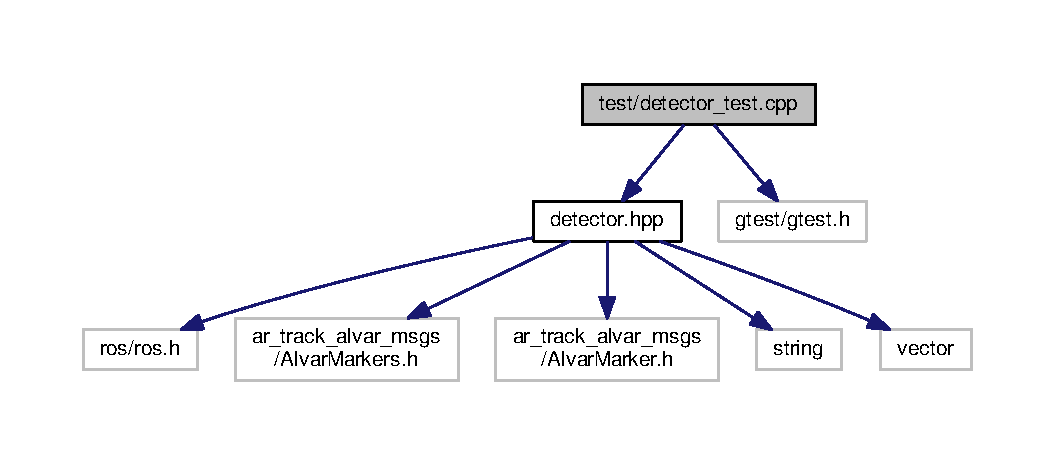
\includegraphics[width=350pt]{detector__test_8cpp__incl}
\end{center}
\end{figure}
\subsection*{Functions}
\begin{DoxyCompactItemize}
\item 
\hyperlink{detector__test_8cpp_a7ced4cdbeca7d328c60d4be9a11ca49e}{T\+E\+ST} (Detector\+Test, test\+No\+Detected\+Markers)
\begin{DoxyCompactList}\small\item\em Test that no markers are detected from a message with no markers. \end{DoxyCompactList}\item 
\hyperlink{detector__test_8cpp_a97193669ca5887d5df9b9b5211c87d69}{T\+E\+ST} (Detector\+Test, test\+Detected\+Markers)
\begin{DoxyCompactList}\small\item\em Test that markers are detected from a message that contains markers. \end{DoxyCompactList}\item 
\hyperlink{detector__test_8cpp_a46128500d8604c71485b7cec202e1ad0}{T\+E\+ST} (Detector\+Test, test\+Is\+Closer\+Than)
\begin{DoxyCompactList}\small\item\em Test that the detector returns the closest of multiple markers. \end{DoxyCompactList}\item 
\hyperlink{detector__test_8cpp_afcc02acf15925a46cec1a7bc4223eb52}{T\+E\+ST} (Detector\+Test, test\+Is\+Marker\+Id\+Valid)
\begin{DoxyCompactList}\small\item\em Test that a marker id is in the list of valid marker ids. \end{DoxyCompactList}\end{DoxyCompactItemize}


\subsection{Detailed Description}
Unit Test for \hyperlink{classDetector}{Detector} class. 

This Source Code Form is subject to the terms of the Mozilla Public License, v. 2.\+0. If a copy of the M\+PL was not distributed with this file, You can obtain one at \href{https://mozilla.org/MPL/2.0/}{\tt https\+://mozilla.\+org/\+M\+P\+L/2.\+0/}.

\begin{DoxyAuthor}{Author}
Pablo Sanhueza, Ryan Cunningham, Andre Gomes 
\end{DoxyAuthor}
\begin{DoxyCopyright}{Copyright}
2019 Pablo Sanhueza, Andre Gomes, Ryan Cunningham 
\end{DoxyCopyright}


\subsection{Function Documentation}
\index{detector\+\_\+test.\+cpp@{detector\+\_\+test.\+cpp}!T\+E\+ST@{T\+E\+ST}}
\index{T\+E\+ST@{T\+E\+ST}!detector\+\_\+test.\+cpp@{detector\+\_\+test.\+cpp}}
\subsubsection[{\texorpdfstring{T\+E\+S\+T(\+Detector\+Test, test\+No\+Detected\+Markers)}{TEST(DetectorTest, testNoDetectedMarkers)}}]{\setlength{\rightskip}{0pt plus 5cm}T\+E\+ST (
\begin{DoxyParamCaption}
\item[{Detector\+Test}]{, }
\item[{test\+No\+Detected\+Markers}]{}
\end{DoxyParamCaption}
)}\hypertarget{detector__test_8cpp_a7ced4cdbeca7d328c60d4be9a11ca49e}{}\label{detector__test_8cpp_a7ced4cdbeca7d328c60d4be9a11ca49e}


Test that no markers are detected from a message with no markers. 


\begin{DoxyParams}[1]{Parameters}
\mbox{\tt in}  & {\em Detector\+Test} & \\
\hline
\mbox{\tt in}  & {\em test\+No\+Detected\+Markers} & \\
\hline
\end{DoxyParams}
\begin{DoxyReturn}{Returns}
none 
\end{DoxyReturn}
create a message with no markers

verify no markers are detected \index{detector\+\_\+test.\+cpp@{detector\+\_\+test.\+cpp}!T\+E\+ST@{T\+E\+ST}}
\index{T\+E\+ST@{T\+E\+ST}!detector\+\_\+test.\+cpp@{detector\+\_\+test.\+cpp}}
\subsubsection[{\texorpdfstring{T\+E\+S\+T(\+Detector\+Test, test\+Detected\+Markers)}{TEST(DetectorTest, testDetectedMarkers)}}]{\setlength{\rightskip}{0pt plus 5cm}T\+E\+ST (
\begin{DoxyParamCaption}
\item[{Detector\+Test}]{, }
\item[{test\+Detected\+Markers}]{}
\end{DoxyParamCaption}
)}\hypertarget{detector__test_8cpp_a97193669ca5887d5df9b9b5211c87d69}{}\label{detector__test_8cpp_a97193669ca5887d5df9b9b5211c87d69}


Test that markers are detected from a message that contains markers. 


\begin{DoxyParams}[1]{Parameters}
\mbox{\tt in}  & {\em Detector\+Test} & \\
\hline
\mbox{\tt in}  & {\em test\+Detected\+Markers} & \\
\hline
\end{DoxyParams}
\begin{DoxyReturn}{Returns}
none 
\end{DoxyReturn}
create a message with 1 marker

create the marker message

verify the marker is detected \index{detector\+\_\+test.\+cpp@{detector\+\_\+test.\+cpp}!T\+E\+ST@{T\+E\+ST}}
\index{T\+E\+ST@{T\+E\+ST}!detector\+\_\+test.\+cpp@{detector\+\_\+test.\+cpp}}
\subsubsection[{\texorpdfstring{T\+E\+S\+T(\+Detector\+Test, test\+Is\+Closer\+Than)}{TEST(DetectorTest, testIsCloserThan)}}]{\setlength{\rightskip}{0pt plus 5cm}T\+E\+ST (
\begin{DoxyParamCaption}
\item[{Detector\+Test}]{, }
\item[{test\+Is\+Closer\+Than}]{}
\end{DoxyParamCaption}
)}\hypertarget{detector__test_8cpp_a46128500d8604c71485b7cec202e1ad0}{}\label{detector__test_8cpp_a46128500d8604c71485b7cec202e1ad0}


Test that the detector returns the closest of multiple markers. 


\begin{DoxyParams}[1]{Parameters}
\mbox{\tt in}  & {\em Detector\+Test} & \\
\hline
\mbox{\tt in}  & {\em test\+Is\+Closer\+Than} & \\
\hline
\end{DoxyParams}
\begin{DoxyReturn}{Returns}
none 
\end{DoxyReturn}
create a message with two markers

the first message will be further away from the robot

the second message will be closer to the robot

verify that the markers are detected

verify that the correct marker is the closest \index{detector\+\_\+test.\+cpp@{detector\+\_\+test.\+cpp}!T\+E\+ST@{T\+E\+ST}}
\index{T\+E\+ST@{T\+E\+ST}!detector\+\_\+test.\+cpp@{detector\+\_\+test.\+cpp}}
\subsubsection[{\texorpdfstring{T\+E\+S\+T(\+Detector\+Test, test\+Is\+Marker\+Id\+Valid)}{TEST(DetectorTest, testIsMarkerIdValid)}}]{\setlength{\rightskip}{0pt plus 5cm}T\+E\+ST (
\begin{DoxyParamCaption}
\item[{Detector\+Test}]{, }
\item[{test\+Is\+Marker\+Id\+Valid}]{}
\end{DoxyParamCaption}
)}\hypertarget{detector__test_8cpp_afcc02acf15925a46cec1a7bc4223eb52}{}\label{detector__test_8cpp_afcc02acf15925a46cec1a7bc4223eb52}


Test that a marker id is in the list of valid marker ids. 


\begin{DoxyParams}[1]{Parameters}
\mbox{\tt in}  & {\em Detector\+Test} & \\
\hline
\mbox{\tt in}  & {\em test\+Is\+Marker\+Id\+Valid} & \\
\hline
\end{DoxyParams}
\begin{DoxyReturn}{Returns}
none 
\end{DoxyReturn}
create valid marker ids

verify that an id in the list of valid ids is valid

verify that an id not in the list of valid ids is invalid 
\hypertarget{modelHandling__test_8cpp}{}\section{test/model\+Handling\+\_\+test.cpp File Reference}
\label{modelHandling__test_8cpp}\index{test/model\+Handling\+\_\+test.\+cpp@{test/model\+Handling\+\_\+test.\+cpp}}


Tests for \hyperlink{classmodelHandling}{model\+Handling} class.  


{\ttfamily \#include $<$gtest/gtest.\+h$>$}\\*
{\ttfamily \#include $<$gazebo\+\_\+msgs/\+Spawn\+Model.\+h$>$}\\*
{\ttfamily \#include $<$gazebo\+\_\+msgs/\+Delete\+Model.\+h$>$}\\*
{\ttfamily \#include $<$ros/ros.\+h$>$}\\*
{\ttfamily \#include $<$ros/package.\+h$>$}\\*
{\ttfamily \#include $<$iostream$>$}\\*
{\ttfamily \#include $<$fstream$>$}\\*
{\ttfamily \#include $<$utility$>$}\\*
{\ttfamily \#include $<$string$>$}\\*
{\ttfamily \#include \char`\"{}model\+Handling.\+hpp\char`\"{}}\\*
Include dependency graph for model\+Handling\+\_\+test.\+cpp\+:
\nopagebreak
\begin{figure}[H]
\begin{center}
\leavevmode
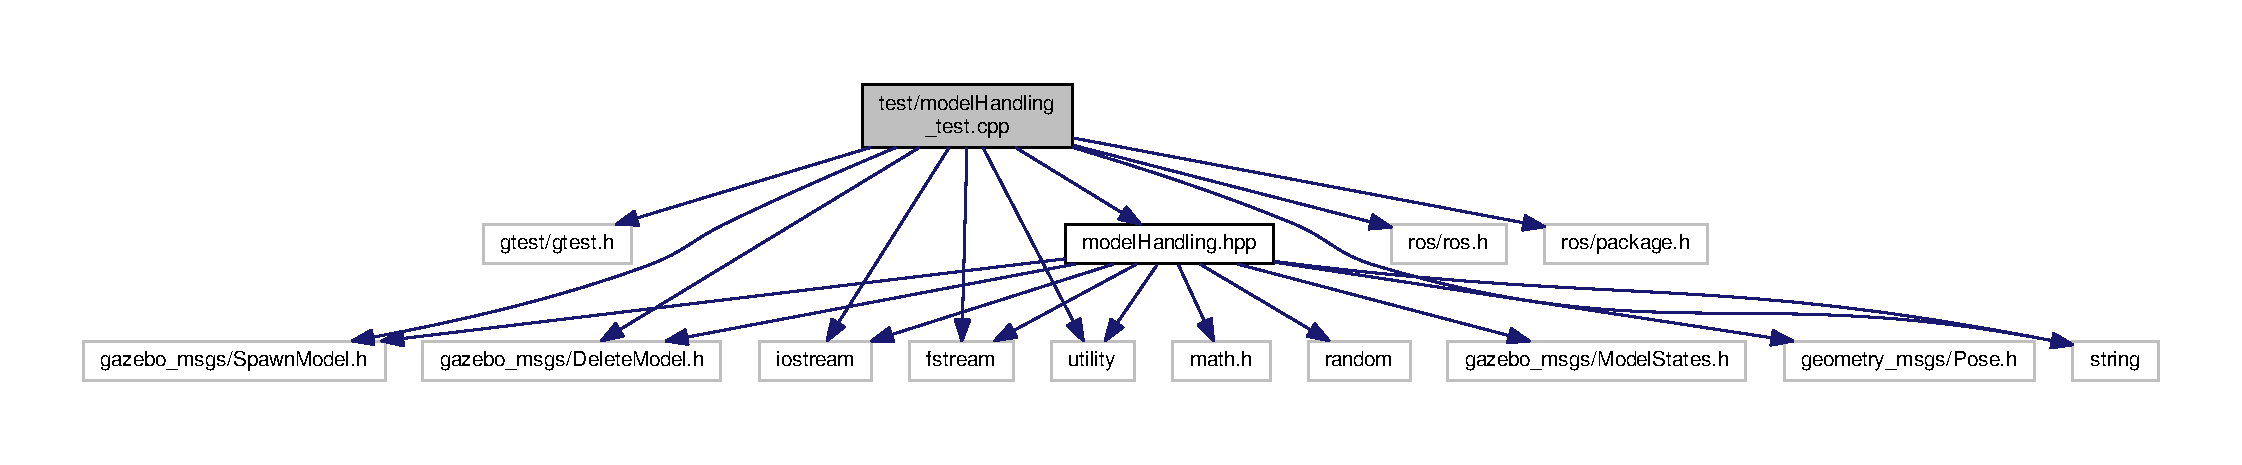
\includegraphics[width=350pt]{modelHandling__test_8cpp__incl}
\end{center}
\end{figure}
\subsection*{Functions}
\begin{DoxyCompactItemize}
\item 
\hyperlink{modelHandling__test_8cpp_a892a556f735170b263f59409a01a277b}{T\+E\+ST} (Model\+Handling\+Test, test\+Get\+Model)
\begin{DoxyCompactList}\small\item\em Test get\+Model() method of \hyperlink{classmodelHandling}{model\+Handling} class. \end{DoxyCompactList}\item 
\hyperlink{modelHandling__test_8cpp_a35c4923e81cd699c2b5eb189657add58}{T\+E\+ST} (Model\+Handling\+Test, test\+Get\+Delete\+Msg)
\begin{DoxyCompactList}\small\item\em Test get\+Delete\+Msg() method of \hyperlink{classmodelHandling}{model\+Handling} class. \end{DoxyCompactList}\end{DoxyCompactItemize}


\subsection{Detailed Description}
Tests for \hyperlink{classmodelHandling}{model\+Handling} class. 

/$\ast$ This Source Code Form is subject to the terms of the Mozilla Public License, v. 2.\+0. If a copy of the M\+PL was not distributed with this file, You can obtain one at \href{https://mozilla.org/MPL/2.0/}{\tt https\+://mozilla.\+org/\+M\+P\+L/2.\+0/}.

\begin{DoxyAuthor}{Author}
Pablo Sanhueza, Ryan Cunningham, Andre Gomes 
\end{DoxyAuthor}
\begin{DoxyCopyright}{Copyright}
2019 Pablo Sanhueza, Ryan Cunningham, Andre Gomes 
\end{DoxyCopyright}


\subsection{Function Documentation}
\index{model\+Handling\+\_\+test.\+cpp@{model\+Handling\+\_\+test.\+cpp}!T\+E\+ST@{T\+E\+ST}}
\index{T\+E\+ST@{T\+E\+ST}!model\+Handling\+\_\+test.\+cpp@{model\+Handling\+\_\+test.\+cpp}}
\subsubsection[{\texorpdfstring{T\+E\+S\+T(\+Model\+Handling\+Test, test\+Get\+Model)}{TEST(ModelHandlingTest, testGetModel)}}]{\setlength{\rightskip}{0pt plus 5cm}T\+E\+ST (
\begin{DoxyParamCaption}
\item[{Model\+Handling\+Test}]{, }
\item[{test\+Get\+Model}]{}
\end{DoxyParamCaption}
)}\hypertarget{modelHandling__test_8cpp_a892a556f735170b263f59409a01a277b}{}\label{modelHandling__test_8cpp_a892a556f735170b263f59409a01a277b}


Test get\+Model() method of \hyperlink{classmodelHandling}{model\+Handling} class. 


\begin{DoxyParams}[1]{Parameters}
\mbox{\tt in}  & {\em Model\+Handling\+Test} & \\
\hline
\mbox{\tt in}  & {\em test\+Get\+Model} & \\
\hline
\end{DoxyParams}
\begin{DoxyReturn}{Returns}
none 
\end{DoxyReturn}
Declase a gazebo\+\_\+msgs of type Spawn\+Model

Retriving file

Giving xml lines of file to model

Setting info to test\+Model

\hyperlink{classmodelHandling}{model\+Handling} object

Calling get\+Model

Making sure the request sets correct parameters \index{model\+Handling\+\_\+test.\+cpp@{model\+Handling\+\_\+test.\+cpp}!T\+E\+ST@{T\+E\+ST}}
\index{T\+E\+ST@{T\+E\+ST}!model\+Handling\+\_\+test.\+cpp@{model\+Handling\+\_\+test.\+cpp}}
\subsubsection[{\texorpdfstring{T\+E\+S\+T(\+Model\+Handling\+Test, test\+Get\+Delete\+Msg)}{TEST(ModelHandlingTest, testGetDeleteMsg)}}]{\setlength{\rightskip}{0pt plus 5cm}T\+E\+ST (
\begin{DoxyParamCaption}
\item[{Model\+Handling\+Test}]{, }
\item[{test\+Get\+Delete\+Msg}]{}
\end{DoxyParamCaption}
)}\hypertarget{modelHandling__test_8cpp_a35c4923e81cd699c2b5eb189657add58}{}\label{modelHandling__test_8cpp_a35c4923e81cd699c2b5eb189657add58}


Test get\+Delete\+Msg() method of \hyperlink{classmodelHandling}{model\+Handling} class. 


\begin{DoxyParams}[1]{Parameters}
\mbox{\tt in}  & {\em Model\+Handling\+Test} & \\
\hline
\mbox{\tt in}  & {\em test\+Get\+Delete\+Msg} & \\
\hline
\end{DoxyParams}
\begin{DoxyReturn}{Returns}
none 
\end{DoxyReturn}
Declaring Delete\+Model request and response for testing

Setting info to test\+Model

\hyperlink{classmodelHandling}{model\+Handling} object

Call get\+Delete\+Msg, pair of response and request to delete a model

Expect false because service call hasn\textquotesingle{}t been used 
\hypertarget{modelHandlingRos__test_8cpp}{}\section{test/model\+Handling\+Ros\+\_\+test.cpp File Reference}
\label{modelHandlingRos__test_8cpp}\index{test/model\+Handling\+Ros\+\_\+test.\+cpp@{test/model\+Handling\+Ros\+\_\+test.\+cpp}}


Test \hyperlink{classmodelHandlingRos}{model\+Handling\+Ros} class.  


{\ttfamily \#include $<$gtest/gtest.\+h$>$}\\*
{\ttfamily \#include $<$ros/ros.\+h$>$}\\*
{\ttfamily \#include $<$gazebo\+\_\+msgs/\+Spawn\+Model.\+h$>$}\\*
{\ttfamily \#include $<$gazebo\+\_\+msgs/\+Delete\+Model.\+h$>$}\\*
{\ttfamily \#include $<$gazebo\+\_\+msgs/\+Model\+States.\+h$>$}\\*
{\ttfamily \#include \char`\"{}model\+Handling\+Ros.\+hpp\char`\"{}}\\*
Include dependency graph for model\+Handling\+Ros\+\_\+test.\+cpp\+:
\nopagebreak
\begin{figure}[H]
\begin{center}
\leavevmode
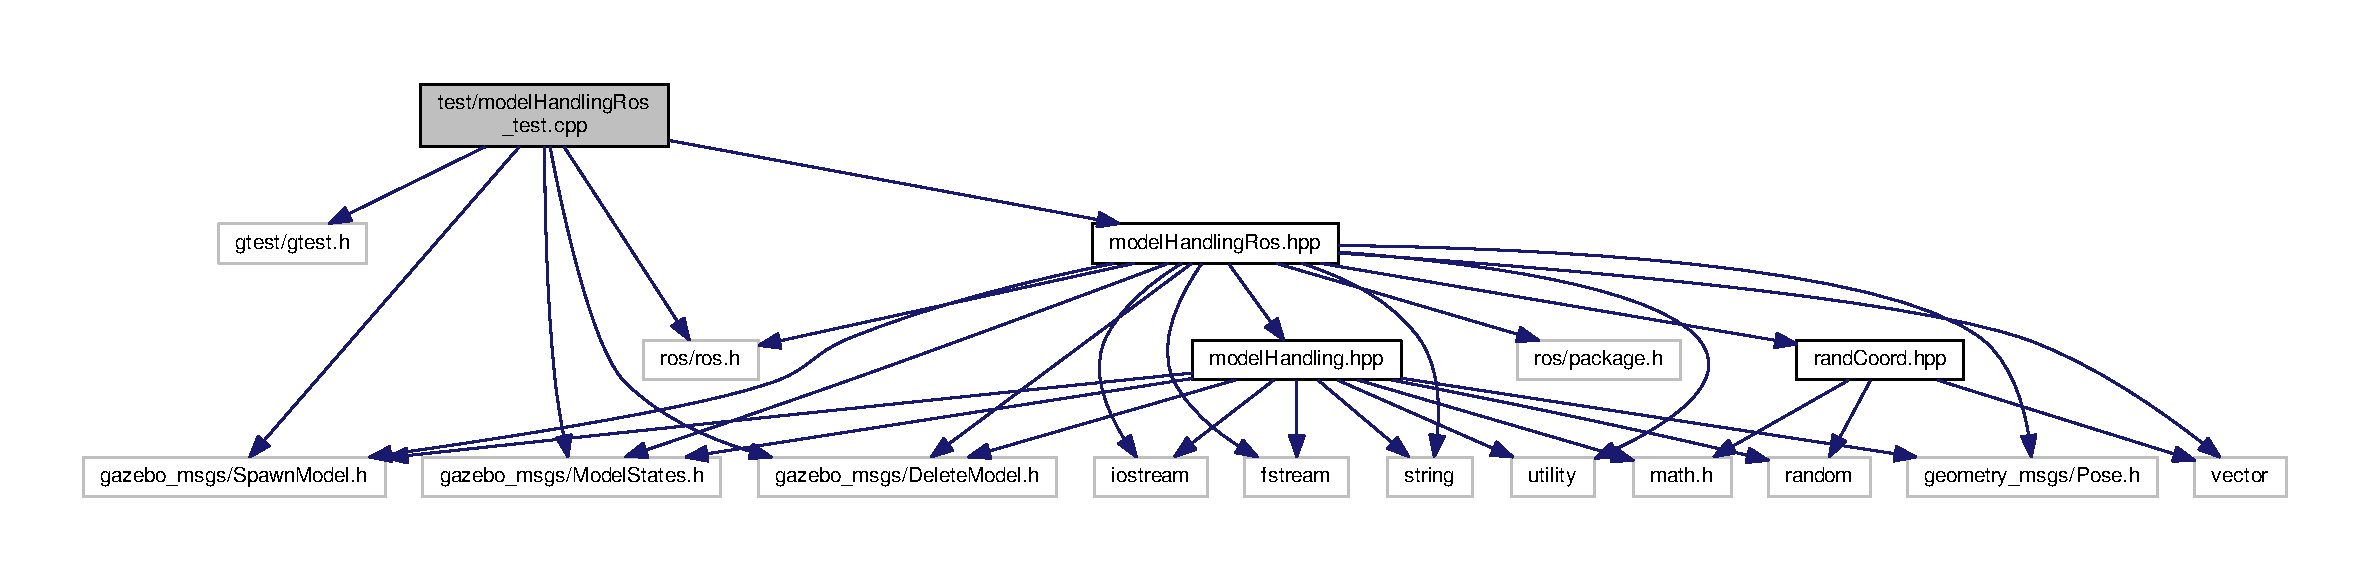
\includegraphics[width=350pt]{modelHandlingRos__test_8cpp__incl}
\end{center}
\end{figure}
\subsection*{Functions}
\begin{DoxyCompactItemize}
\item 
\hyperlink{modelHandlingRos__test_8cpp_a34378977272508299952ce572823c5dd}{T\+E\+ST} (Model\+Handling\+Ros\+Test, test\+Constructor\+Service\+Clients)
\begin{DoxyCompactList}\small\item\em Test Constructor of \hyperlink{classmodelHandlingRos}{model\+Handling\+Ros} class. \end{DoxyCompactList}\item 
\hyperlink{modelHandlingRos__test_8cpp_aea8a96433214140546248f9d27644df9}{T\+E\+ST} (Model\+Handling\+Ros\+Test, test\+Add\+Models)
\begin{DoxyCompactList}\small\item\em Test add\+Models() method of \hyperlink{classmodelHandlingRos}{model\+Handling\+Ros} class. \end{DoxyCompactList}\item 
\hyperlink{modelHandlingRos__test_8cpp_a18a91296018727a82ea7d933c631fd95}{T\+E\+ST} (Model\+Handling\+Ros\+Test, test\+Remove\+Models)
\begin{DoxyCompactList}\small\item\em Test remove\+Models() of \hyperlink{classmodelHandlingRos}{model\+Handling\+Ros} class. \end{DoxyCompactList}\end{DoxyCompactItemize}


\subsection{Detailed Description}
Test \hyperlink{classmodelHandlingRos}{model\+Handling\+Ros} class. 

/$\ast$ This Source Code Form is subject to the terms of the Mozilla Public License, v. 2.\+0. If a copy of the M\+PL was not distributed with this file, You can obtain one at \href{https://mozilla.org/MPL/2.0/}{\tt https\+://mozilla.\+org/\+M\+P\+L/2.\+0/}.

\begin{DoxyAuthor}{Author}
Pablo Sanhueza, Ryan Cunningham, Andre Gomes 
\end{DoxyAuthor}
\begin{DoxyCopyright}{Copyright}
2019 Pablo Sanhueza, Ryan Cunningham, Andre Gomes 
\end{DoxyCopyright}


\subsection{Function Documentation}
\index{model\+Handling\+Ros\+\_\+test.\+cpp@{model\+Handling\+Ros\+\_\+test.\+cpp}!T\+E\+ST@{T\+E\+ST}}
\index{T\+E\+ST@{T\+E\+ST}!model\+Handling\+Ros\+\_\+test.\+cpp@{model\+Handling\+Ros\+\_\+test.\+cpp}}
\subsubsection[{\texorpdfstring{T\+E\+S\+T(\+Model\+Handling\+Ros\+Test, test\+Constructor\+Service\+Clients)}{TEST(ModelHandlingRosTest, testConstructorServiceClients)}}]{\setlength{\rightskip}{0pt plus 5cm}T\+E\+ST (
\begin{DoxyParamCaption}
\item[{Model\+Handling\+Ros\+Test}]{, }
\item[{test\+Constructor\+Service\+Clients}]{}
\end{DoxyParamCaption}
)}\hypertarget{modelHandlingRos__test_8cpp_a34378977272508299952ce572823c5dd}{}\label{modelHandlingRos__test_8cpp_a34378977272508299952ce572823c5dd}


Test Constructor of \hyperlink{classmodelHandlingRos}{model\+Handling\+Ros} class. 


\begin{DoxyParams}[1]{Parameters}
\mbox{\tt in}  & {\em Model\+Handling\+Ros\+Test} & \\
\hline
\mbox{\tt in}  & {\em test\+Constructor\+Service\+Clients} & \\
\hline
\end{DoxyParams}
\begin{DoxyReturn}{Returns}
none 
\end{DoxyReturn}
Services used

\hyperlink{classmodelHandlingRos}{model\+Handling\+Ros} object -\/ pass ros package name

Get Service Clients

Make sure that Service\+Client Exists

Run tests \index{model\+Handling\+Ros\+\_\+test.\+cpp@{model\+Handling\+Ros\+\_\+test.\+cpp}!T\+E\+ST@{T\+E\+ST}}
\index{T\+E\+ST@{T\+E\+ST}!model\+Handling\+Ros\+\_\+test.\+cpp@{model\+Handling\+Ros\+\_\+test.\+cpp}}
\subsubsection[{\texorpdfstring{T\+E\+S\+T(\+Model\+Handling\+Ros\+Test, test\+Add\+Models)}{TEST(ModelHandlingRosTest, testAddModels)}}]{\setlength{\rightskip}{0pt plus 5cm}T\+E\+ST (
\begin{DoxyParamCaption}
\item[{Model\+Handling\+Ros\+Test}]{, }
\item[{test\+Add\+Models}]{}
\end{DoxyParamCaption}
)}\hypertarget{modelHandlingRos__test_8cpp_aea8a96433214140546248f9d27644df9}{}\label{modelHandlingRos__test_8cpp_aea8a96433214140546248f9d27644df9}


Test add\+Models() method of \hyperlink{classmodelHandlingRos}{model\+Handling\+Ros} class. 


\begin{DoxyParams}[1]{Parameters}
\mbox{\tt in}  & {\em Model\+Handling\+Ros\+Test} & \\
\hline
\mbox{\tt in}  & {\em test\+Add\+Models} & \\
\hline
\end{DoxyParams}
\begin{DoxyReturn}{Returns}
none 
\end{DoxyReturn}
\hyperlink{classmodelHandlingRos}{model\+Handling\+Ros} object

parameters of model

Add models to world

Get public variable from model\+Handling\+Class

Run test \index{model\+Handling\+Ros\+\_\+test.\+cpp@{model\+Handling\+Ros\+\_\+test.\+cpp}!T\+E\+ST@{T\+E\+ST}}
\index{T\+E\+ST@{T\+E\+ST}!model\+Handling\+Ros\+\_\+test.\+cpp@{model\+Handling\+Ros\+\_\+test.\+cpp}}
\subsubsection[{\texorpdfstring{T\+E\+S\+T(\+Model\+Handling\+Ros\+Test, test\+Remove\+Models)}{TEST(ModelHandlingRosTest, testRemoveModels)}}]{\setlength{\rightskip}{0pt plus 5cm}T\+E\+ST (
\begin{DoxyParamCaption}
\item[{Model\+Handling\+Ros\+Test}]{, }
\item[{test\+Remove\+Models}]{}
\end{DoxyParamCaption}
)}\hypertarget{modelHandlingRos__test_8cpp_a18a91296018727a82ea7d933c631fd95}{}\label{modelHandlingRos__test_8cpp_a18a91296018727a82ea7d933c631fd95}


Test remove\+Models() of \hyperlink{classmodelHandlingRos}{model\+Handling\+Ros} class. 


\begin{DoxyParams}[1]{Parameters}
\mbox{\tt in}  & {\em Model\+Handling\+Ros\+Test} & \\
\hline
\mbox{\tt in}  & {\em test\+Remove\+Models} & \\
\hline
\end{DoxyParams}
\begin{DoxyReturn}{Returns}
none 
\end{DoxyReturn}
\hyperlink{classmodelHandlingRos}{model\+Handling\+Ros} object

Model id to be deleted

Remove model from world

Get Delete Service\+Client

Run test 
\hypertarget{randCoord__test_8cpp}{}\section{test/rand\+Coord\+\_\+test.cpp File Reference}
\label{randCoord__test_8cpp}\index{test/rand\+Coord\+\_\+test.\+cpp@{test/rand\+Coord\+\_\+test.\+cpp}}


Test of \hyperlink{classrandCoord}{rand\+Coord} class.  


{\ttfamily \#include \char`\"{}rand\+Coord.\+hpp\char`\"{}}\\*
{\ttfamily \#include $<$gtest/gtest.\+h$>$}\\*
{\ttfamily \#include $<$vector$>$}\\*
Include dependency graph for rand\+Coord\+\_\+test.\+cpp\+:
\nopagebreak
\begin{figure}[H]
\begin{center}
\leavevmode
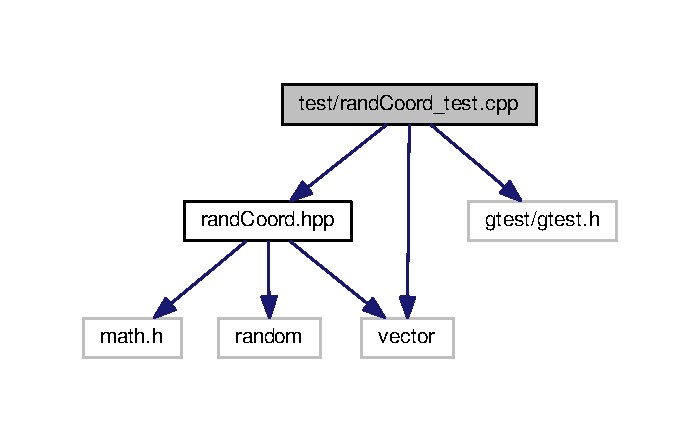
\includegraphics[width=336pt]{randCoord__test_8cpp__incl}
\end{center}
\end{figure}
\subsection*{Functions}
\begin{DoxyCompactItemize}
\item 
\hyperlink{randCoord__test_8cpp_a7abe7cc0c8c860294f6530c89a406027}{T\+E\+ST} (Rand\+Coord\+Test, test\+Constructor)
\begin{DoxyCompactList}\small\item\em Test Constructor of \hyperlink{classrandCoord}{rand\+Coord} class. \end{DoxyCompactList}\item 
\hyperlink{randCoord__test_8cpp_ae46e8f086c59bd19f4968758a882484d}{T\+E\+ST} (Detector\+Test, test\+RandX)
\begin{DoxyCompactList}\small\item\em Test rand\+X() method of \hyperlink{classrandCoord}{rand\+Coord} class. \end{DoxyCompactList}\item 
\hyperlink{randCoord__test_8cpp_a47e722cd12ec4893bbaf34ed251f170c}{T\+E\+ST} (Detector\+Test, test\+RandY)
\begin{DoxyCompactList}\small\item\em Test randy() method of \hyperlink{classrandCoord}{rand\+Coord} class. \end{DoxyCompactList}\end{DoxyCompactItemize}


\subsection{Detailed Description}
Test of \hyperlink{classrandCoord}{rand\+Coord} class. 

/$\ast$ This Source Code Form is subject to the terms of the Mozilla Public License, v. 2.\+0. If a copy of the M\+PL was not distributed with this file, You can obtain one at \href{https://mozilla.org/MPL/2.0/}{\tt https\+://mozilla.\+org/\+M\+P\+L/2.\+0/}.

\begin{DoxyAuthor}{Author}
Pablo Sanhueza, Ryan Cunningham, Andre Gomes 
\end{DoxyAuthor}
\begin{DoxyCopyright}{Copyright}
2019 Pablo Sanhueza, Ryan Cunningham, Andre Gomes 
\end{DoxyCopyright}


\subsection{Function Documentation}
\index{rand\+Coord\+\_\+test.\+cpp@{rand\+Coord\+\_\+test.\+cpp}!T\+E\+ST@{T\+E\+ST}}
\index{T\+E\+ST@{T\+E\+ST}!rand\+Coord\+\_\+test.\+cpp@{rand\+Coord\+\_\+test.\+cpp}}
\subsubsection[{\texorpdfstring{T\+E\+S\+T(\+Rand\+Coord\+Test, test\+Constructor)}{TEST(RandCoordTest, testConstructor)}}]{\setlength{\rightskip}{0pt plus 5cm}T\+E\+ST (
\begin{DoxyParamCaption}
\item[{Rand\+Coord\+Test}]{, }
\item[{test\+Constructor}]{}
\end{DoxyParamCaption}
)}\hypertarget{randCoord__test_8cpp_a7abe7cc0c8c860294f6530c89a406027}{}\label{randCoord__test_8cpp_a7abe7cc0c8c860294f6530c89a406027}


Test Constructor of \hyperlink{classrandCoord}{rand\+Coord} class. 


\begin{DoxyParams}[1]{Parameters}
\mbox{\tt in}  & {\em Rand\+Coord\+Test} & \\
\hline
\mbox{\tt in}  & {\em test\+Constructor} & \\
\hline
\end{DoxyParams}
\begin{DoxyReturn}{Returns}
none 
\end{DoxyReturn}
Center of map vector

\hyperlink{classrandCoord}{rand\+Coord} object

Check if constructor sets members \index{rand\+Coord\+\_\+test.\+cpp@{rand\+Coord\+\_\+test.\+cpp}!T\+E\+ST@{T\+E\+ST}}
\index{T\+E\+ST@{T\+E\+ST}!rand\+Coord\+\_\+test.\+cpp@{rand\+Coord\+\_\+test.\+cpp}}
\subsubsection[{\texorpdfstring{T\+E\+S\+T(\+Detector\+Test, test\+Rand\+X)}{TEST(DetectorTest, testRandX)}}]{\setlength{\rightskip}{0pt plus 5cm}T\+E\+ST (
\begin{DoxyParamCaption}
\item[{Detector\+Test}]{, }
\item[{test\+RandX}]{}
\end{DoxyParamCaption}
)}\hypertarget{randCoord__test_8cpp_ae46e8f086c59bd19f4968758a882484d}{}\label{randCoord__test_8cpp_ae46e8f086c59bd19f4968758a882484d}


Test rand\+X() method of \hyperlink{classrandCoord}{rand\+Coord} class. 


\begin{DoxyParams}[1]{Parameters}
\mbox{\tt in}  & {\em Detector\+Test} & \\
\hline
\mbox{\tt in}  & {\em test\+RandX} & \\
\hline
\end{DoxyParams}
\begin{DoxyReturn}{Returns}
none 
\end{DoxyReturn}
Center of map vector

\hyperlink{classrandCoord}{rand\+Coord} object

Creating random x coords

Check if random x coord is within map range \index{rand\+Coord\+\_\+test.\+cpp@{rand\+Coord\+\_\+test.\+cpp}!T\+E\+ST@{T\+E\+ST}}
\index{T\+E\+ST@{T\+E\+ST}!rand\+Coord\+\_\+test.\+cpp@{rand\+Coord\+\_\+test.\+cpp}}
\subsubsection[{\texorpdfstring{T\+E\+S\+T(\+Detector\+Test, test\+Rand\+Y)}{TEST(DetectorTest, testRandY)}}]{\setlength{\rightskip}{0pt plus 5cm}T\+E\+ST (
\begin{DoxyParamCaption}
\item[{Detector\+Test}]{, }
\item[{test\+RandY}]{}
\end{DoxyParamCaption}
)}\hypertarget{randCoord__test_8cpp_a47e722cd12ec4893bbaf34ed251f170c}{}\label{randCoord__test_8cpp_a47e722cd12ec4893bbaf34ed251f170c}


Test randy() method of \hyperlink{classrandCoord}{rand\+Coord} class. 


\begin{DoxyParams}[1]{Parameters}
\mbox{\tt in}  & {\em Detector\+Test} & \\
\hline
\mbox{\tt in}  & {\em test\+RandY} & \\
\hline
\end{DoxyParams}
\begin{DoxyReturn}{Returns}
none 
\end{DoxyReturn}
Center of map vector

\hyperlink{classrandCoord}{rand\+Coord} object

Creating random y coords

Check if random y coord is within map range 
\hypertarget{walkRobot__test_8cpp}{}\section{test/walk\+Robot\+\_\+test.cpp File Reference}
\label{walkRobot__test_8cpp}\index{test/walk\+Robot\+\_\+test.\+cpp@{test/walk\+Robot\+\_\+test.\+cpp}}


Source code for the implementation of \hyperlink{classwalkRobot}{walk\+Robot} class.  


{\ttfamily \#include $<$ros/ros.\+h$>$}\\*
{\ttfamily \#include $<$unistd.\+h$>$}\\*
{\ttfamily \#include $<$sensor\+\_\+msgs/\+Laser\+Scan.\+h$>$}\\*
{\ttfamily \#include $<$geometry\+\_\+msgs/\+Twist.\+h$>$}\\*
{\ttfamily \#include $<$gtest/gtest.\+h$>$}\\*
{\ttfamily \#include \char`\"{}walk\+Robot\+Ros.\+hpp\char`\"{}}\\*
Include dependency graph for walk\+Robot\+\_\+test.\+cpp\+:
\nopagebreak
\begin{figure}[H]
\begin{center}
\leavevmode
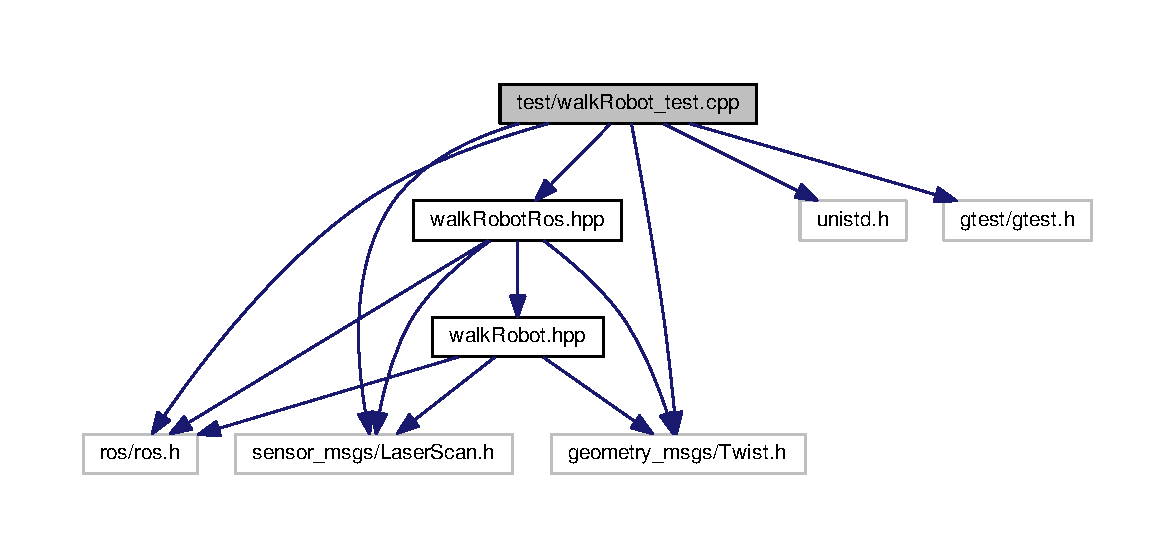
\includegraphics[width=350pt]{walkRobot__test_8cpp__incl}
\end{center}
\end{figure}
\subsection*{Functions}
\begin{DoxyCompactItemize}
\item 
\hyperlink{walkRobot__test_8cpp_a272d5f1681a60881885351ac427fa530}{T\+E\+ST} (walk\+Robot\+Test, Test\+Obstacle\+Found)
\begin{DoxyCompactList}\small\item\em Test remove\+Models() of \hyperlink{classmodelHandlingRos}{model\+Handling\+Ros} class. \end{DoxyCompactList}\item 
\hyperlink{walkRobot__test_8cpp_afc06f3d1ffdda6bf23309b642857ab6e}{T\+E\+ST} (walk\+Robot\+Test, Test\+Linear\+Velocity)
\begin{DoxyCompactList}\small\item\em Test remove\+Models() of \hyperlink{classmodelHandlingRos}{model\+Handling\+Ros} class. \end{DoxyCompactList}\item 
\hyperlink{walkRobot__test_8cpp_a76fb2796dc5b8ae434675db4dda99ee5}{T\+E\+ST} (walk\+Robot\+Test, Test\+Positive\+Angular\+Velocity)
\begin{DoxyCompactList}\small\item\em Test remove\+Models() of \hyperlink{classmodelHandlingRos}{model\+Handling\+Ros} class. \end{DoxyCompactList}\item 
\hyperlink{walkRobot__test_8cpp_ad45bd6ce9747a7a9d75ca3bea931ff63}{T\+E\+ST} (walk\+Robot\+Test, Test\+Negative\+Angular\+Velocity)
\begin{DoxyCompactList}\small\item\em Test remove\+Models() of \hyperlink{classmodelHandlingRos}{model\+Handling\+Ros} class. \end{DoxyCompactList}\end{DoxyCompactItemize}


\subsection{Detailed Description}
Source code for the implementation of \hyperlink{classwalkRobot}{walk\+Robot} class. 

/$\ast$ This Source Code Form is subject to the terms of the Mozilla Public License, v. 2.\+0. If a copy of the M\+PL was not distributed with this file, You can obtain one at \href{https://mozilla.org/MPL/2.0/}{\tt https\+://mozilla.\+org/\+M\+P\+L/2.\+0/}.

\begin{DoxyAuthor}{Author}
Pablo Sanhueza, Ryan Cunningham, Andre Gomes 
\end{DoxyAuthor}
\begin{DoxyCopyright}{Copyright}
2019 Pablo Sanhueza, Ryan Cunningham, Andre Gomes 
\end{DoxyCopyright}


\subsection{Function Documentation}
\index{walk\+Robot\+\_\+test.\+cpp@{walk\+Robot\+\_\+test.\+cpp}!T\+E\+ST@{T\+E\+ST}}
\index{T\+E\+ST@{T\+E\+ST}!walk\+Robot\+\_\+test.\+cpp@{walk\+Robot\+\_\+test.\+cpp}}
\subsubsection[{\texorpdfstring{T\+E\+S\+T(walk\+Robot\+Test, Test\+Obstacle\+Found)}{TEST(walkRobotTest, TestObstacleFound)}}]{\setlength{\rightskip}{0pt plus 5cm}T\+E\+ST (
\begin{DoxyParamCaption}
\item[{walk\+Robot\+Test}]{, }
\item[{Test\+Obstacle\+Found}]{}
\end{DoxyParamCaption}
)}\hypertarget{walkRobot__test_8cpp_a272d5f1681a60881885351ac427fa530}{}\label{walkRobot__test_8cpp_a272d5f1681a60881885351ac427fa530}


Test remove\+Models() of \hyperlink{classmodelHandlingRos}{model\+Handling\+Ros} class. 


\begin{DoxyParams}[1]{Parameters}
\mbox{\tt in}  & {\em walk\+Robot\+Test} & \\
\hline
\mbox{\tt in}  & {\em Test\+Obstacle\+Found} & \\
\hline
\end{DoxyParams}
\begin{DoxyReturn}{Returns}
none 
\end{DoxyReturn}
Creating Object of \hyperlink{classwalkRobot}{walk\+Robot}

setting obstacle equal true

Calling method from \hyperlink{classwalkRobot}{walk\+Robot}

Expected linear velocity to avoid obstacle \index{walk\+Robot\+\_\+test.\+cpp@{walk\+Robot\+\_\+test.\+cpp}!T\+E\+ST@{T\+E\+ST}}
\index{T\+E\+ST@{T\+E\+ST}!walk\+Robot\+\_\+test.\+cpp@{walk\+Robot\+\_\+test.\+cpp}}
\subsubsection[{\texorpdfstring{T\+E\+S\+T(walk\+Robot\+Test, Test\+Linear\+Velocity)}{TEST(walkRobotTest, TestLinearVelocity)}}]{\setlength{\rightskip}{0pt plus 5cm}T\+E\+ST (
\begin{DoxyParamCaption}
\item[{walk\+Robot\+Test}]{, }
\item[{Test\+Linear\+Velocity}]{}
\end{DoxyParamCaption}
)}\hypertarget{walkRobot__test_8cpp_afc06f3d1ffdda6bf23309b642857ab6e}{}\label{walkRobot__test_8cpp_afc06f3d1ffdda6bf23309b642857ab6e}


Test remove\+Models() of \hyperlink{classmodelHandlingRos}{model\+Handling\+Ros} class. 


\begin{DoxyParams}[1]{Parameters}
\mbox{\tt in}  & {\em walk\+Robot\+Test} & \\
\hline
\mbox{\tt in}  & {\em Test\+Linear\+Velocity} & \\
\hline
\end{DoxyParams}
\begin{DoxyReturn}{Returns}
none 
\end{DoxyReturn}
Creating Object of \hyperlink{classwalkRobot}{walk\+Robot}

setting obstacle equal false

setting linear velocity

Calling method from \hyperlink{classwalkRobot}{walk\+Robot}

Expect linear velocity equal 1 \index{walk\+Robot\+\_\+test.\+cpp@{walk\+Robot\+\_\+test.\+cpp}!T\+E\+ST@{T\+E\+ST}}
\index{T\+E\+ST@{T\+E\+ST}!walk\+Robot\+\_\+test.\+cpp@{walk\+Robot\+\_\+test.\+cpp}}
\subsubsection[{\texorpdfstring{T\+E\+S\+T(walk\+Robot\+Test, Test\+Positive\+Angular\+Velocity)}{TEST(walkRobotTest, TestPositiveAngularVelocity)}}]{\setlength{\rightskip}{0pt plus 5cm}T\+E\+ST (
\begin{DoxyParamCaption}
\item[{walk\+Robot\+Test}]{, }
\item[{Test\+Positive\+Angular\+Velocity}]{}
\end{DoxyParamCaption}
)}\hypertarget{walkRobot__test_8cpp_a76fb2796dc5b8ae434675db4dda99ee5}{}\label{walkRobot__test_8cpp_a76fb2796dc5b8ae434675db4dda99ee5}


Test remove\+Models() of \hyperlink{classmodelHandlingRos}{model\+Handling\+Ros} class. 


\begin{DoxyParams}[1]{Parameters}
\mbox{\tt in}  & {\em walk\+Robot\+Test} & \\
\hline
\mbox{\tt in}  & {\em Test\+Positive\+Angular\+Velocity} & \\
\hline
\end{DoxyParams}
\begin{DoxyReturn}{Returns}
none 
\end{DoxyReturn}
Creating Object of \hyperlink{classwalkRobot}{walk\+Robot}

setting obstacle equal false

setting action to positive velocity

Calling method from \hyperlink{classwalkRobot}{walk\+Robot}

Expect linear velocity equal 0.\+5 \index{walk\+Robot\+\_\+test.\+cpp@{walk\+Robot\+\_\+test.\+cpp}!T\+E\+ST@{T\+E\+ST}}
\index{T\+E\+ST@{T\+E\+ST}!walk\+Robot\+\_\+test.\+cpp@{walk\+Robot\+\_\+test.\+cpp}}
\subsubsection[{\texorpdfstring{T\+E\+S\+T(walk\+Robot\+Test, Test\+Negative\+Angular\+Velocity)}{TEST(walkRobotTest, TestNegativeAngularVelocity)}}]{\setlength{\rightskip}{0pt plus 5cm}T\+E\+ST (
\begin{DoxyParamCaption}
\item[{walk\+Robot\+Test}]{, }
\item[{Test\+Negative\+Angular\+Velocity}]{}
\end{DoxyParamCaption}
)}\hypertarget{walkRobot__test_8cpp_ad45bd6ce9747a7a9d75ca3bea931ff63}{}\label{walkRobot__test_8cpp_ad45bd6ce9747a7a9d75ca3bea931ff63}


Test remove\+Models() of \hyperlink{classmodelHandlingRos}{model\+Handling\+Ros} class. 


\begin{DoxyParams}[1]{Parameters}
\mbox{\tt in}  & {\em walk\+Robot\+Test} & \\
\hline
\mbox{\tt in}  & {\em Test\+Negative\+Angular\+Velocity} & \\
\hline
\end{DoxyParams}
\begin{DoxyReturn}{Returns}
none 
\end{DoxyReturn}
Creating Object of \hyperlink{classwalkRobot}{walk\+Robot}

setting obstacle equal false

setting action to negative velocity

Calling method from \hyperlink{classwalkRobot}{walk\+Robot}

Expect linear velocity equal -\/0.\+5 
\hypertarget{walkRobotRos__test_8cpp}{}\section{test/walk\+Robot\+Ros\+\_\+test.cpp File Reference}
\label{walkRobotRos__test_8cpp}\index{test/walk\+Robot\+Ros\+\_\+test.\+cpp@{test/walk\+Robot\+Ros\+\_\+test.\+cpp}}


Source code for the implementation of \hyperlink{classwalkRobotRos}{walk\+Robot\+Ros} tests.  


{\ttfamily \#include \char`\"{}walk\+Robot\+Ros.\+hpp\char`\"{}}\\*
{\ttfamily \#include $<$ros/ros.\+h$>$}\\*
{\ttfamily \#include $<$sensor\+\_\+msgs/\+Laser\+Scan.\+h$>$}\\*
{\ttfamily \#include $<$geometry\+\_\+msgs/\+Twist.\+h$>$}\\*
{\ttfamily \#include $<$gtest/gtest.\+h$>$}\\*
{\ttfamily \#include $<$unistd.\+h$>$}\\*
Include dependency graph for walk\+Robot\+Ros\+\_\+test.\+cpp\+:
\nopagebreak
\begin{figure}[H]
\begin{center}
\leavevmode
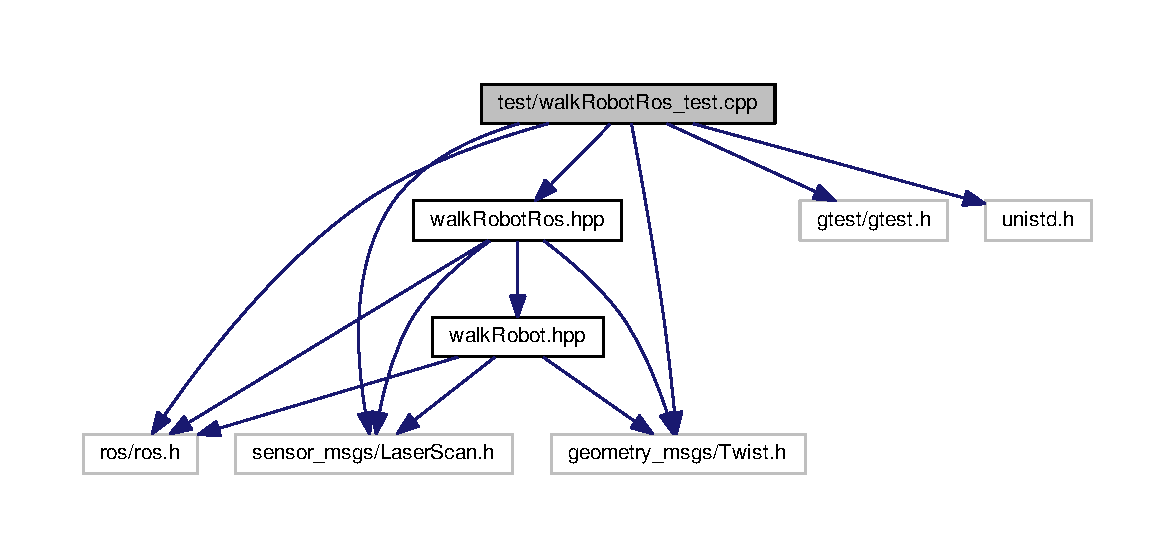
\includegraphics[width=350pt]{walkRobotRos__test_8cpp__incl}
\end{center}
\end{figure}
\subsection*{Classes}
\begin{DoxyCompactItemize}
\item 
struct \hyperlink{structTestSubHelper}{Test\+Sub\+Helper}
\begin{DoxyCompactList}\small\item\em Struct to count the callback function was called. \end{DoxyCompactList}\end{DoxyCompactItemize}
\subsection*{Functions}
\begin{DoxyCompactItemize}
\item 
\hyperlink{walkRobotRos__test_8cpp_ab43be7d8ed68d1ced5a0cd174ae5a949}{T\+E\+ST} (walk\+Robot\+Ros\+Test, Test\+Laser\+Sensor\+Callback)
\begin{DoxyCompactList}\small\item\em Test remove\+Models() of \hyperlink{classmodelHandlingRos}{model\+Handling\+Ros} class. \end{DoxyCompactList}\item 
\hyperlink{walkRobotRos__test_8cpp_acc41388b081ff9dbd332ad19698be076}{T\+E\+ST} (walk\+Robot\+Ros\+Test, Test\+Walk\+Robot\+Ros)
\begin{DoxyCompactList}\small\item\em Test remove\+Models() of \hyperlink{classmodelHandlingRos}{model\+Handling\+Ros} class. \end{DoxyCompactList}\end{DoxyCompactItemize}


\subsection{Detailed Description}
Source code for the implementation of \hyperlink{classwalkRobotRos}{walk\+Robot\+Ros} tests. 

/$\ast$ This Source Code Form is subject to the terms of the Mozilla Public License, v. 2.\+0. If a copy of the M\+PL was not distributed with this file, You can obtain one at \href{https://mozilla.org/MPL/2.0/}{\tt https\+://mozilla.\+org/\+M\+P\+L/2.\+0/}.

\begin{DoxyAuthor}{Author}
Pablo Sanhueza, Ryan Cunningham, Andre Gomes 
\end{DoxyAuthor}
\begin{DoxyCopyright}{Copyright}
2019 Pablo Sanhueza, Ryan Cunningham, Andre Gomes 
\end{DoxyCopyright}


\subsection{Function Documentation}
\index{walk\+Robot\+Ros\+\_\+test.\+cpp@{walk\+Robot\+Ros\+\_\+test.\+cpp}!T\+E\+ST@{T\+E\+ST}}
\index{T\+E\+ST@{T\+E\+ST}!walk\+Robot\+Ros\+\_\+test.\+cpp@{walk\+Robot\+Ros\+\_\+test.\+cpp}}
\subsubsection[{\texorpdfstring{T\+E\+S\+T(walk\+Robot\+Ros\+Test, Test\+Laser\+Sensor\+Callback)}{TEST(walkRobotRosTest, TestLaserSensorCallback)}}]{\setlength{\rightskip}{0pt plus 5cm}T\+E\+ST (
\begin{DoxyParamCaption}
\item[{walk\+Robot\+Ros\+Test}]{, }
\item[{Test\+Laser\+Sensor\+Callback}]{}
\end{DoxyParamCaption}
)}\hypertarget{walkRobotRos__test_8cpp_ab43be7d8ed68d1ced5a0cd174ae5a949}{}\label{walkRobotRos__test_8cpp_ab43be7d8ed68d1ced5a0cd174ae5a949}


Test remove\+Models() of \hyperlink{classmodelHandlingRos}{model\+Handling\+Ros} class. 


\begin{DoxyParams}[1]{Parameters}
\mbox{\tt in}  & {\em walk\+Robot\+Ros\+Test} & \\
\hline
\mbox{\tt in}  & {\em Test\+Laser\+Sensor\+Callback} & \\
\hline
\end{DoxyParams}
\begin{DoxyReturn}{Returns}
none 
\end{DoxyReturn}
nodehandle R\+OS

Generating publisher to topic /scan

Generating a laser mensage to be published at topic /scan

Setting the values og ranges to 0.\+1 to be detected as obstacle

Create object of class \hyperlink{classwalkRobotRos}{walk\+Robot\+Ros}

loop Rate

publish test

Break loop after 11 iterations to generate new random value

Test if obstacle was detected \index{walk\+Robot\+Ros\+\_\+test.\+cpp@{walk\+Robot\+Ros\+\_\+test.\+cpp}!T\+E\+ST@{T\+E\+ST}}
\index{T\+E\+ST@{T\+E\+ST}!walk\+Robot\+Ros\+\_\+test.\+cpp@{walk\+Robot\+Ros\+\_\+test.\+cpp}}
\subsubsection[{\texorpdfstring{T\+E\+S\+T(walk\+Robot\+Ros\+Test, Test\+Walk\+Robot\+Ros)}{TEST(walkRobotRosTest, TestWalkRobotRos)}}]{\setlength{\rightskip}{0pt plus 5cm}T\+E\+ST (
\begin{DoxyParamCaption}
\item[{walk\+Robot\+Ros\+Test}]{, }
\item[{Test\+Walk\+Robot\+Ros}]{}
\end{DoxyParamCaption}
)}\hypertarget{walkRobotRos__test_8cpp_acc41388b081ff9dbd332ad19698be076}{}\label{walkRobotRos__test_8cpp_acc41388b081ff9dbd332ad19698be076}


Test remove\+Models() of \hyperlink{classmodelHandlingRos}{model\+Handling\+Ros} class. 


\begin{DoxyParams}[1]{Parameters}
\mbox{\tt in}  & {\em walk\+Robot\+Ros\+Test} & \\
\hline
\mbox{\tt in}  & {\em Test\+Walk\+Robot\+Ros} & \\
\hline
\end{DoxyParams}
\begin{DoxyReturn}{Returns}
none 
\end{DoxyReturn}
Initilize instance of a struct

Create object of class \hyperlink{classwalkRobotRos}{walk\+Robot\+Ros}

nodehandle R\+OS

Generating a velocity subscriber

publish test 
%--- End generated contents ---

% Index
\backmatter
\newpage
\phantomsection
\clearemptydoublepage
\addcontentsline{toc}{chapter}{Index}
\printindex

\end{document}
